\FloatBarrier
\subsection{The event-plane resolution}

\begin{figure}[ht]
    \centering
    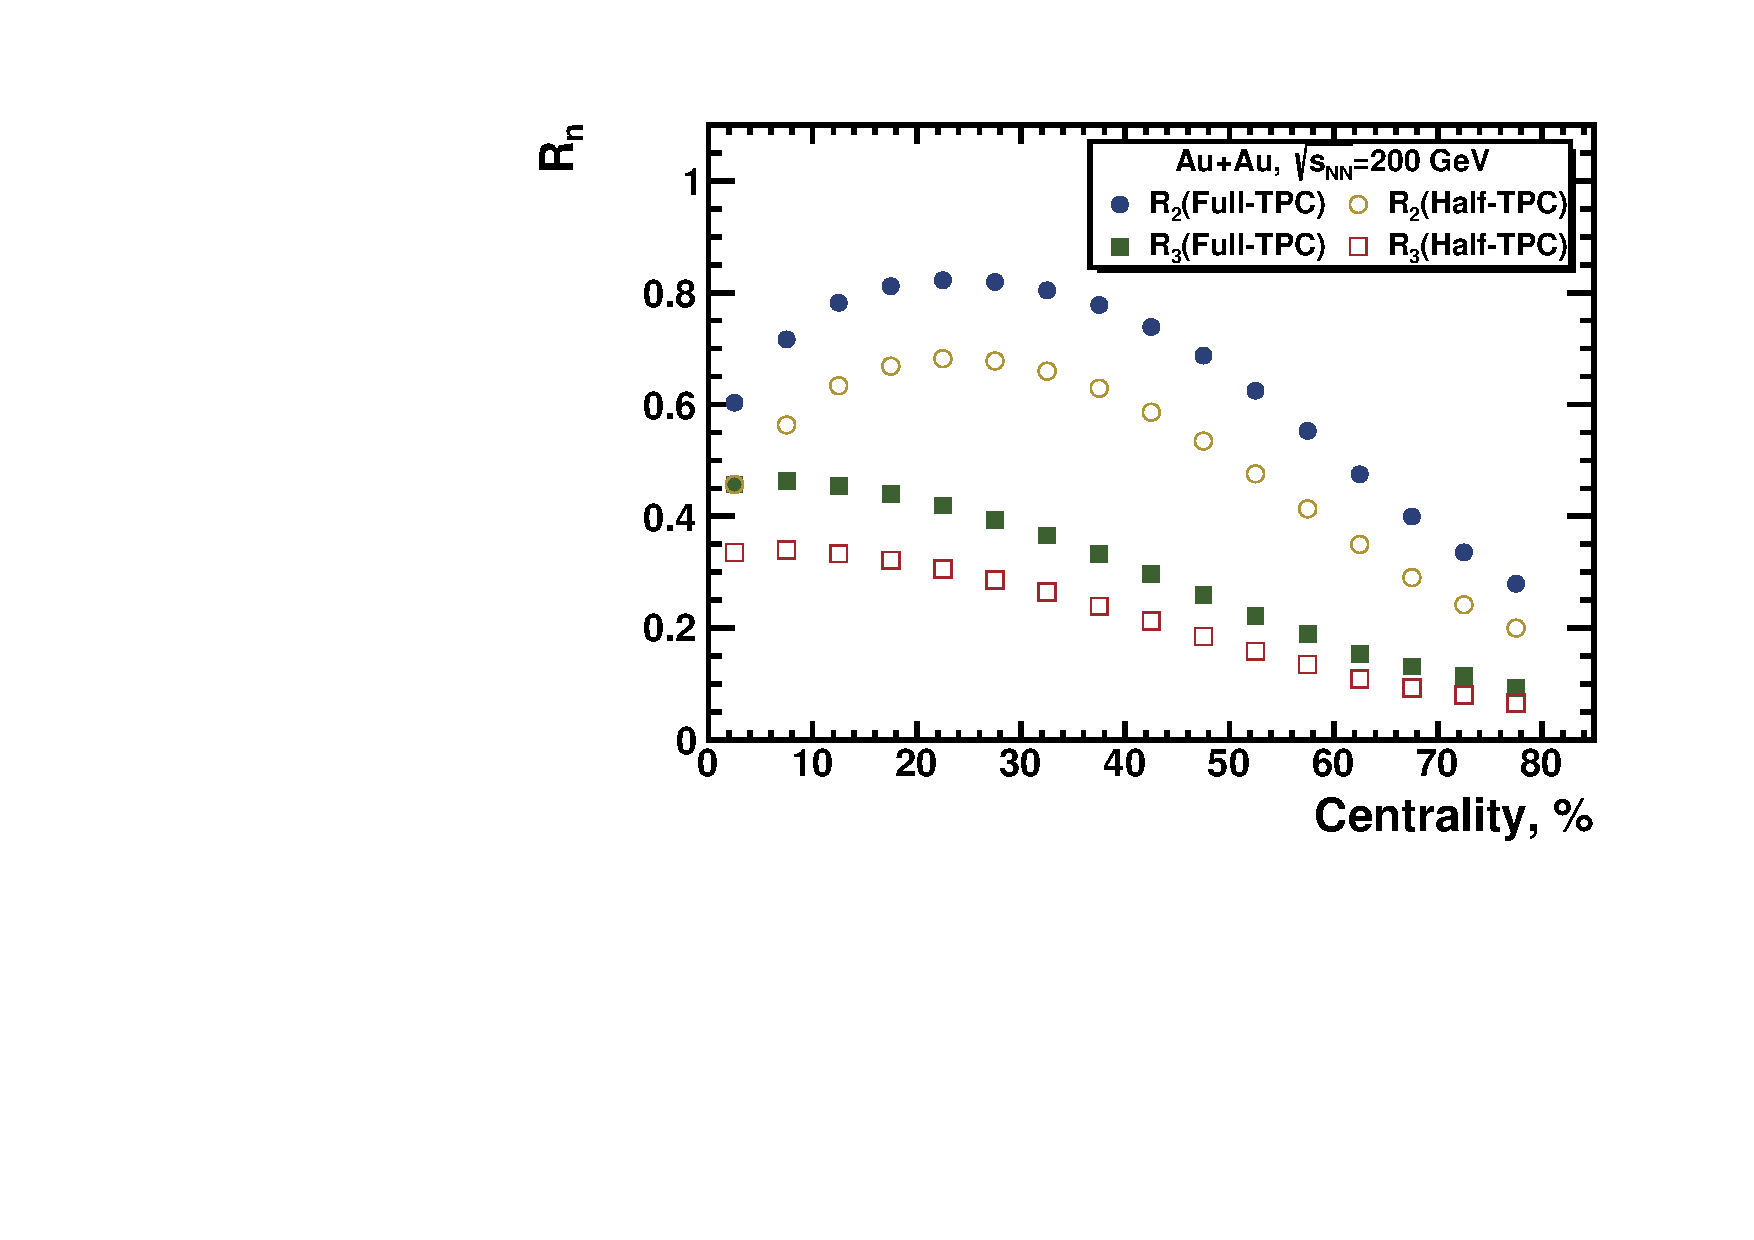
\includegraphics[width=0.7\linewidth]{Figures/ResEPFullHalfvn.pdf}
    \caption{The event-plane resolution correction factor calculated for \AuAu\ collisions at \sNN\ = 200 GeV using $\eta$-sub method as a function of centrality. Results presented for half \TPC\ (open markers) and for the full \TPC\ approximation \cite{Ollitrault:1992bk,Ollitrault:1993ba} (filled markers).}
    \label{fig:res_EP}
\end{figure}

\FloatBarrier
\subsection{Anisotropic flow for the charged hadrons}

\FloatBarrier
\subsubsection{Elliptic flow}

\begin{figure}[ht]
    \begin{subfigure}{.49\textwidth}
        \centering
        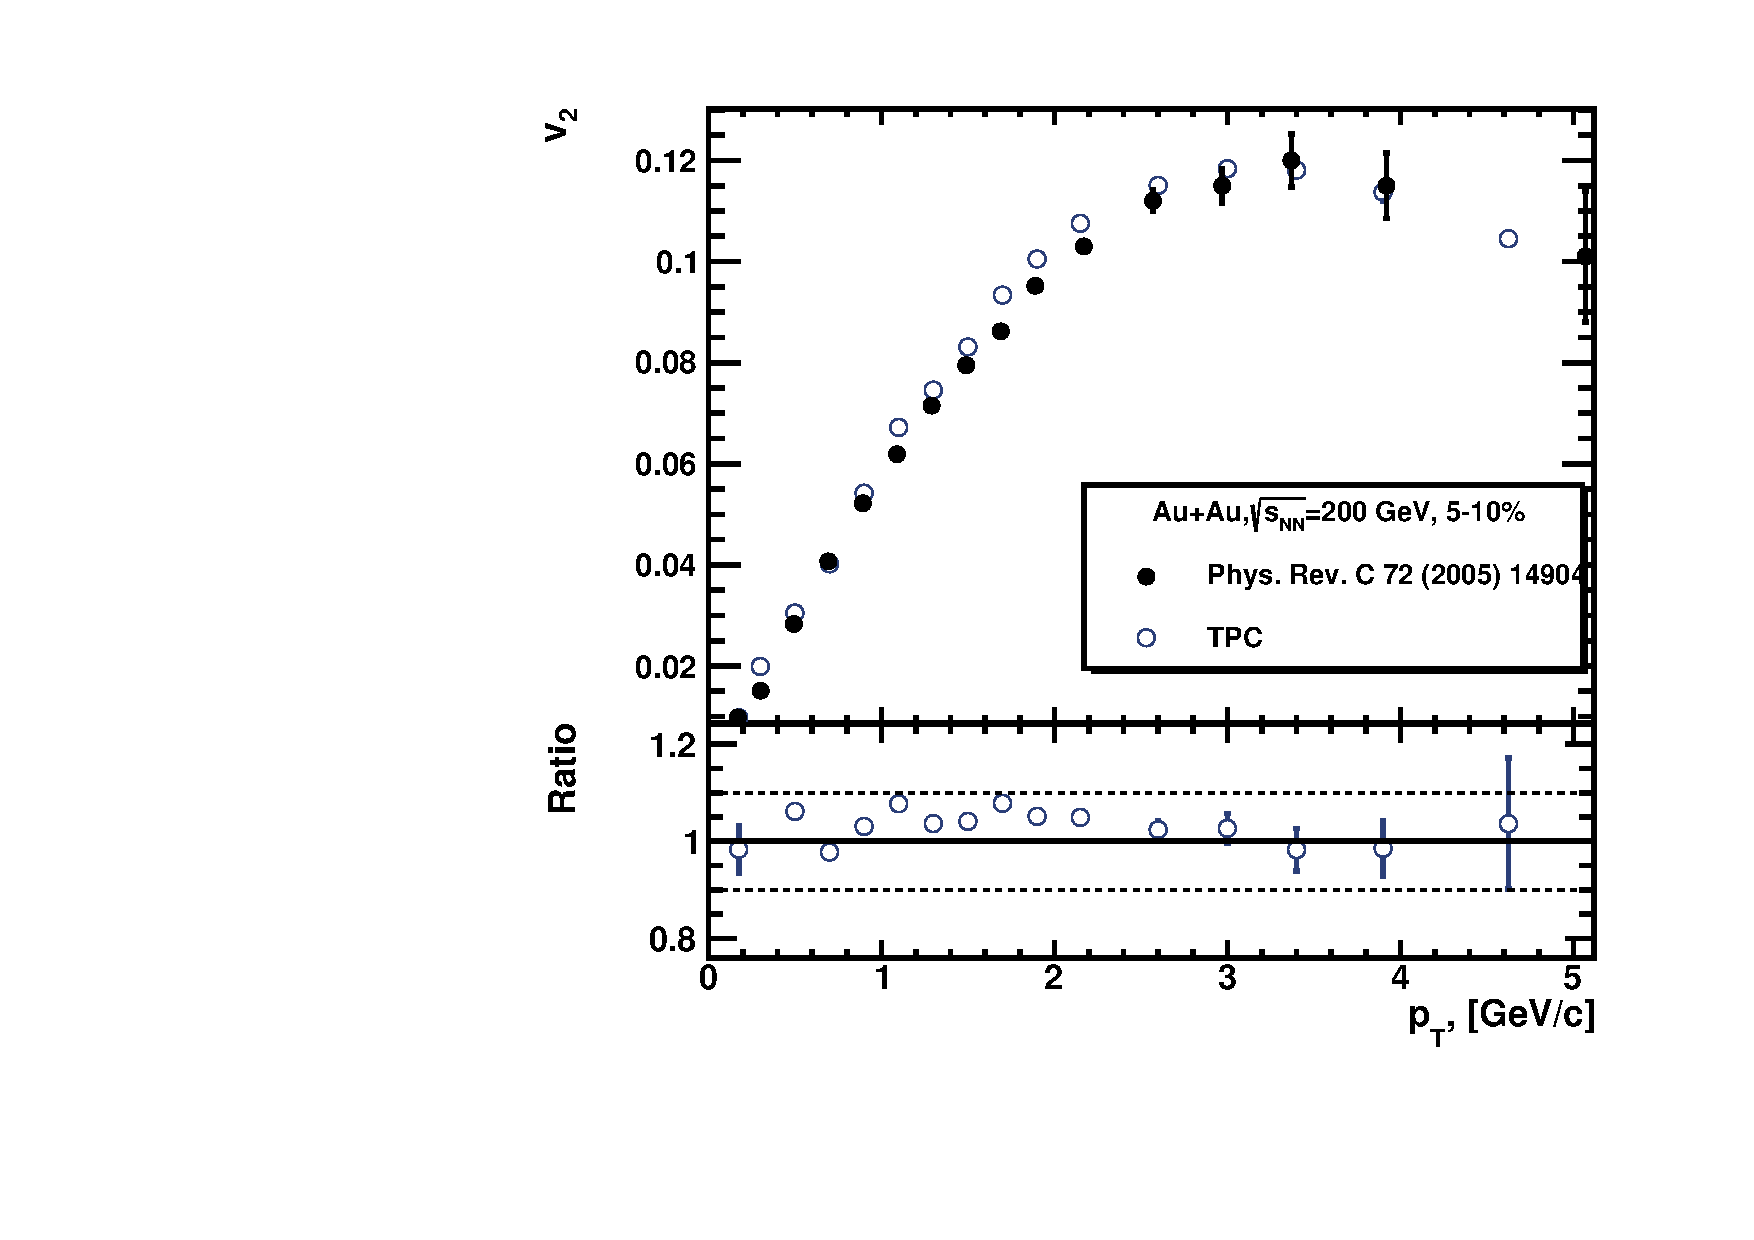
\includegraphics[width=1.\linewidth]{Figures/v2_charged_hadrons_pt_cent1.pdf}
        %\caption{a}
    \end{subfigure}
    \begin{subfigure}{.49\textwidth}
        \centering
        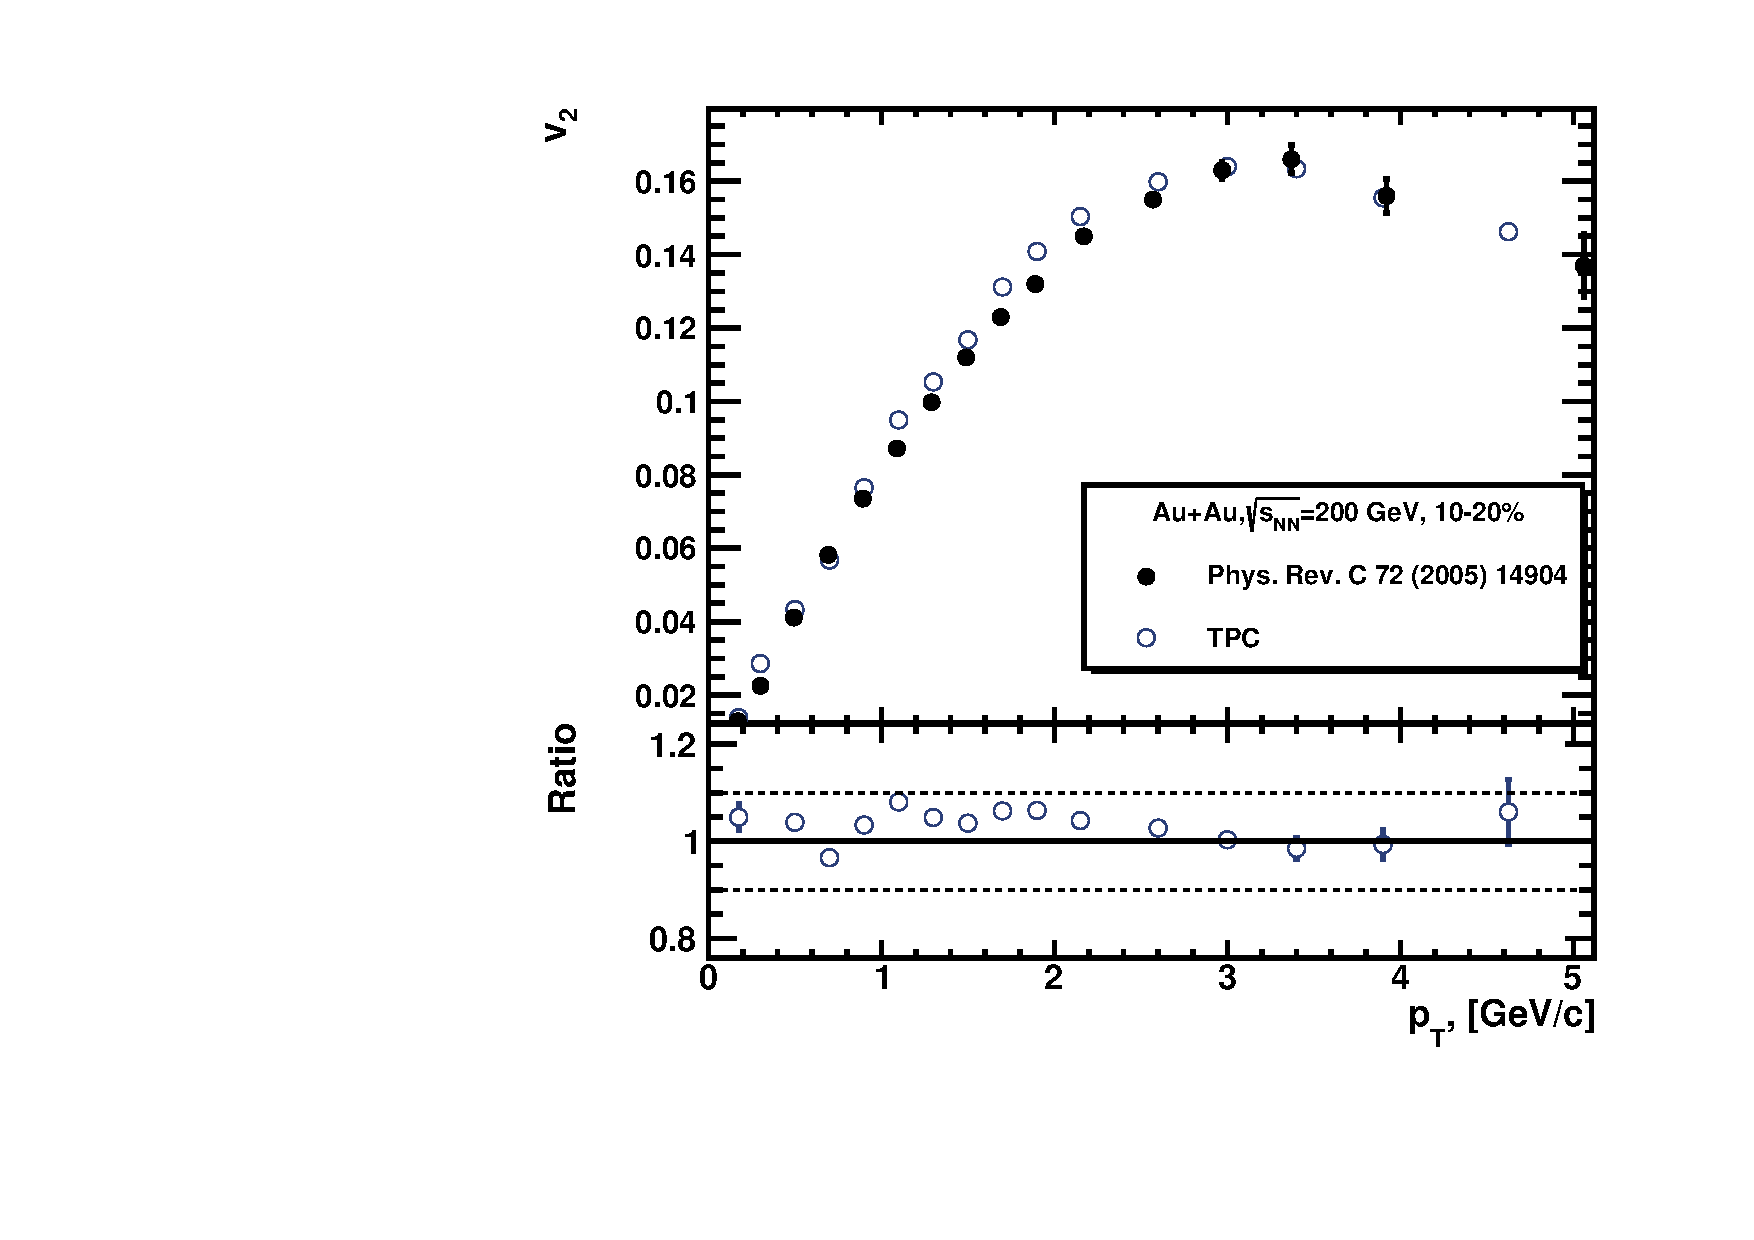
\includegraphics[width=1.\linewidth]{Figures/v2_charged_hadrons_pt_cent2.pdf}
        %\caption{b}
    \end{subfigure}
    \\
    \begin{subfigure}{.49\textwidth}
        \centering
        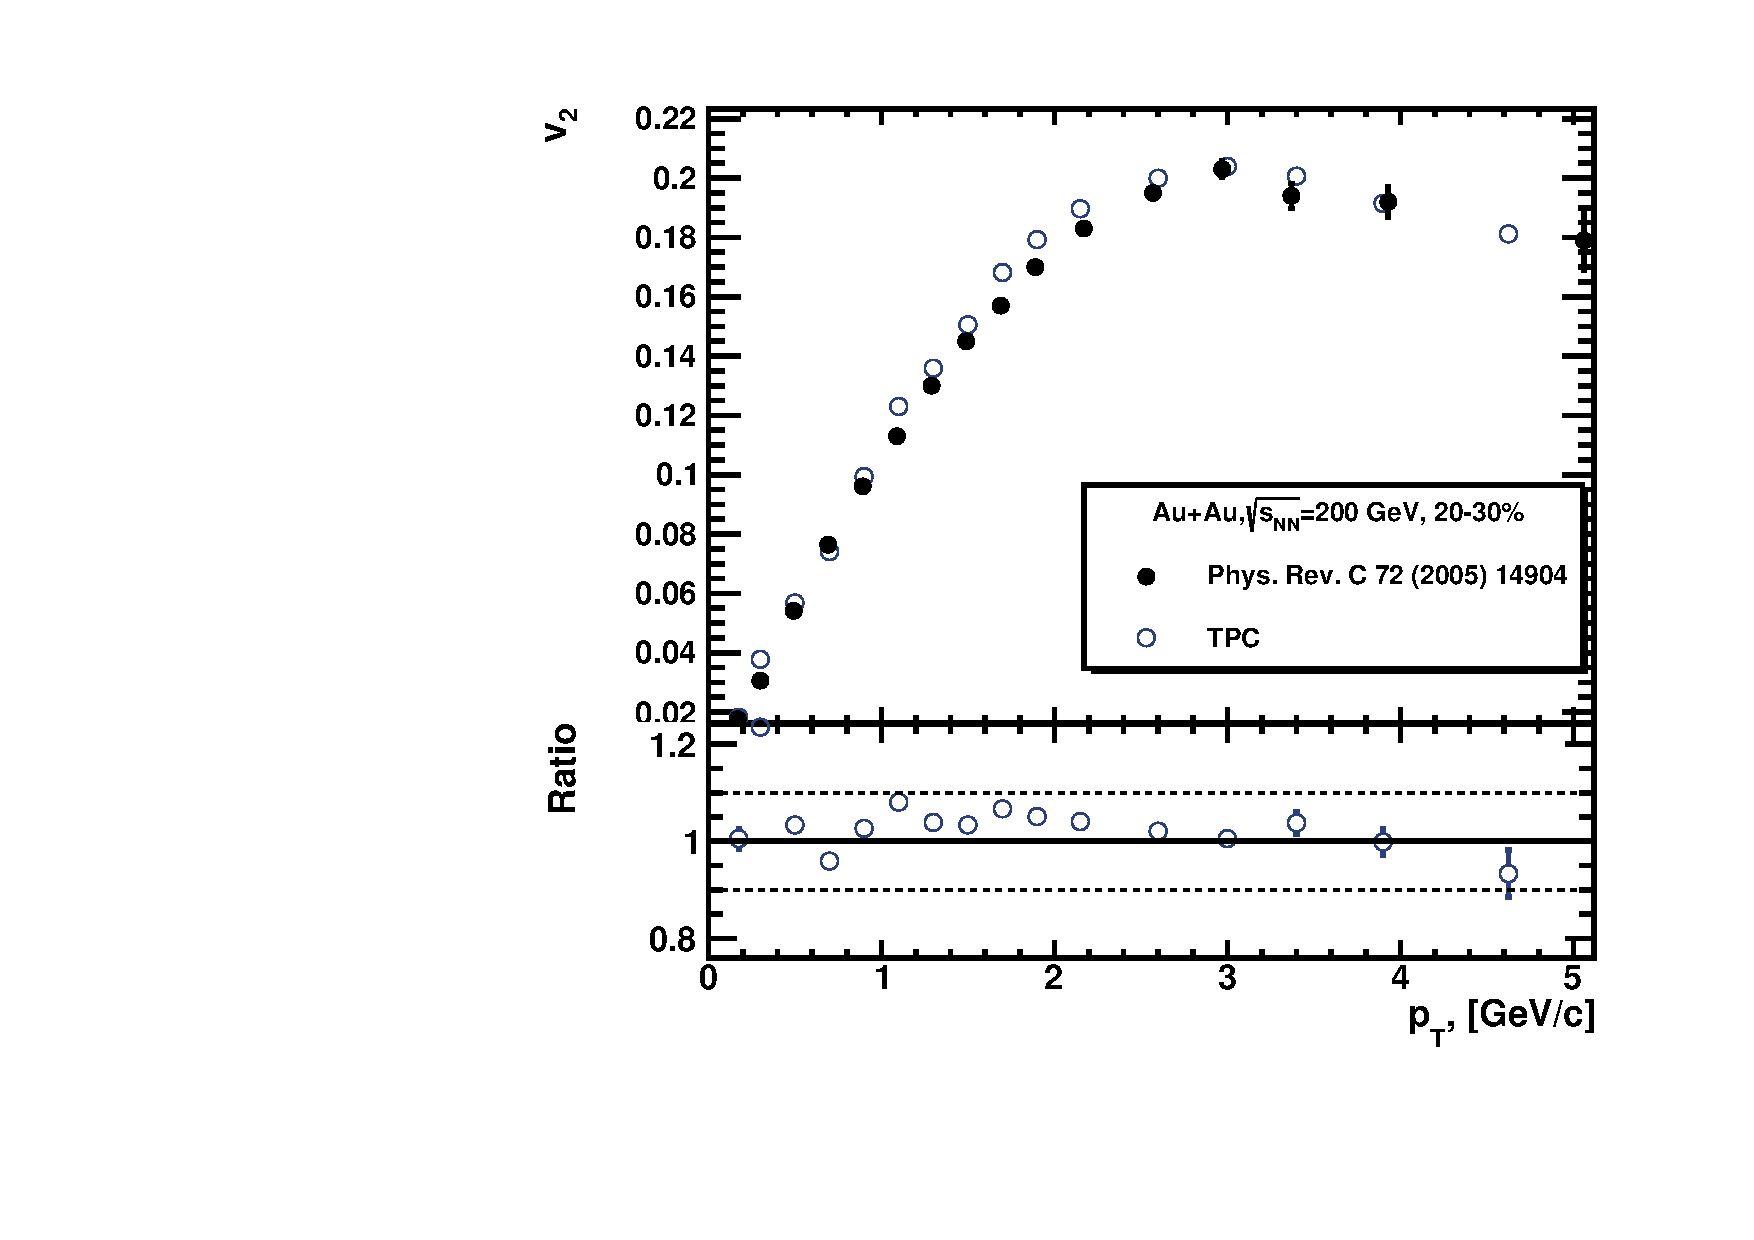
\includegraphics[width=1.\linewidth]{Figures/v2_charged_hadrons_pt_cent3.pdf}
        %\caption{a}
    \end{subfigure}
    \begin{subfigure}{.49\textwidth}
        \centering
        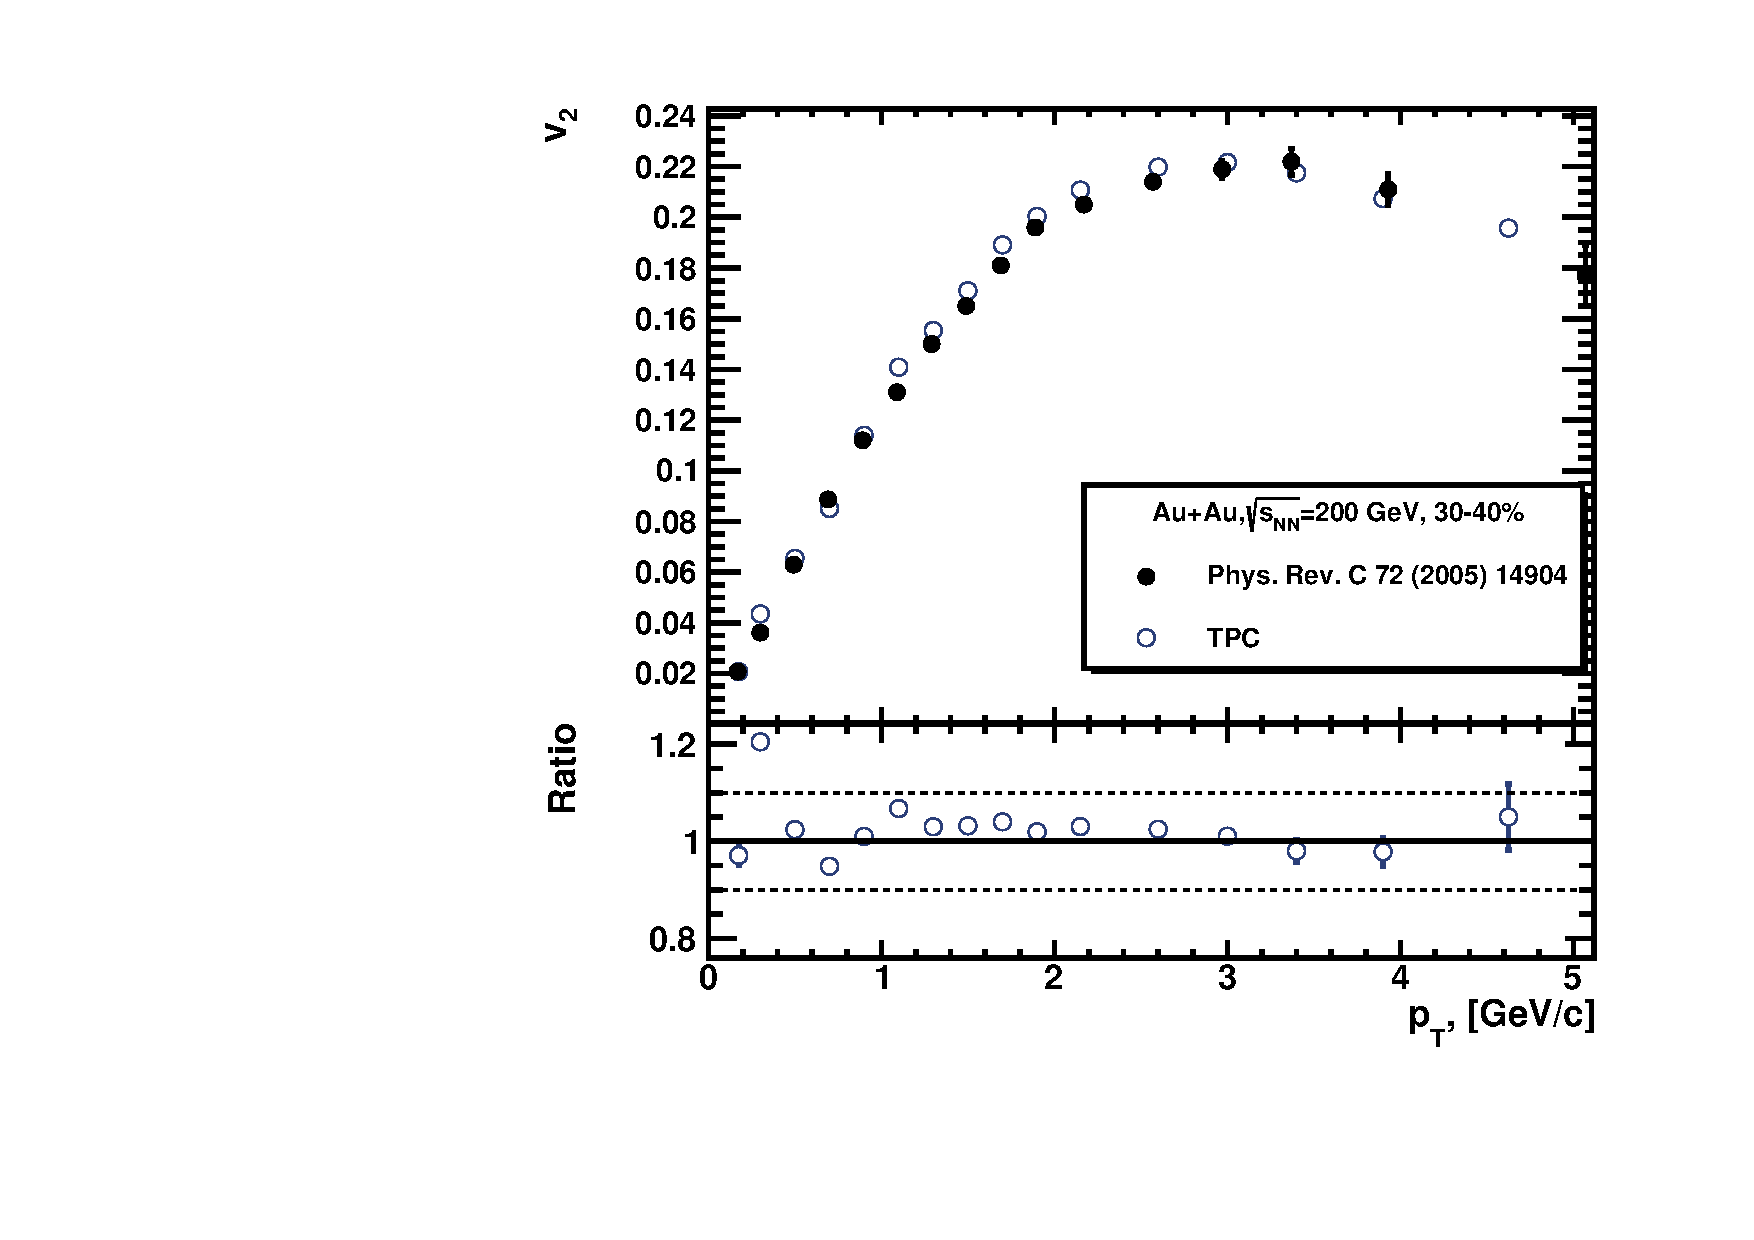
\includegraphics[width=1.\linewidth]{Figures/v2_charged_hadrons_pt_cent4.pdf}
        %\caption{b}
    \end{subfigure}
    \label{fig:v2_EP_CH}
    \caption{Charged hadron $v_2(p_T)$ for 5-10\% (upper left), 10-20\% (upper right), 20-30\% (bottom left) and 30-40 \% (bottom right) centrality classes in \AuAu\ collisions at \sNN\ = 200 GeV. Results were compared with published data \cite{Adams:2004bi}.}
\end{figure}

\FloatBarrier
\subsubsection{Triangular flow}

\begin{figure}[ht]
    \begin{subfigure}{.49\textwidth}
        \centering
        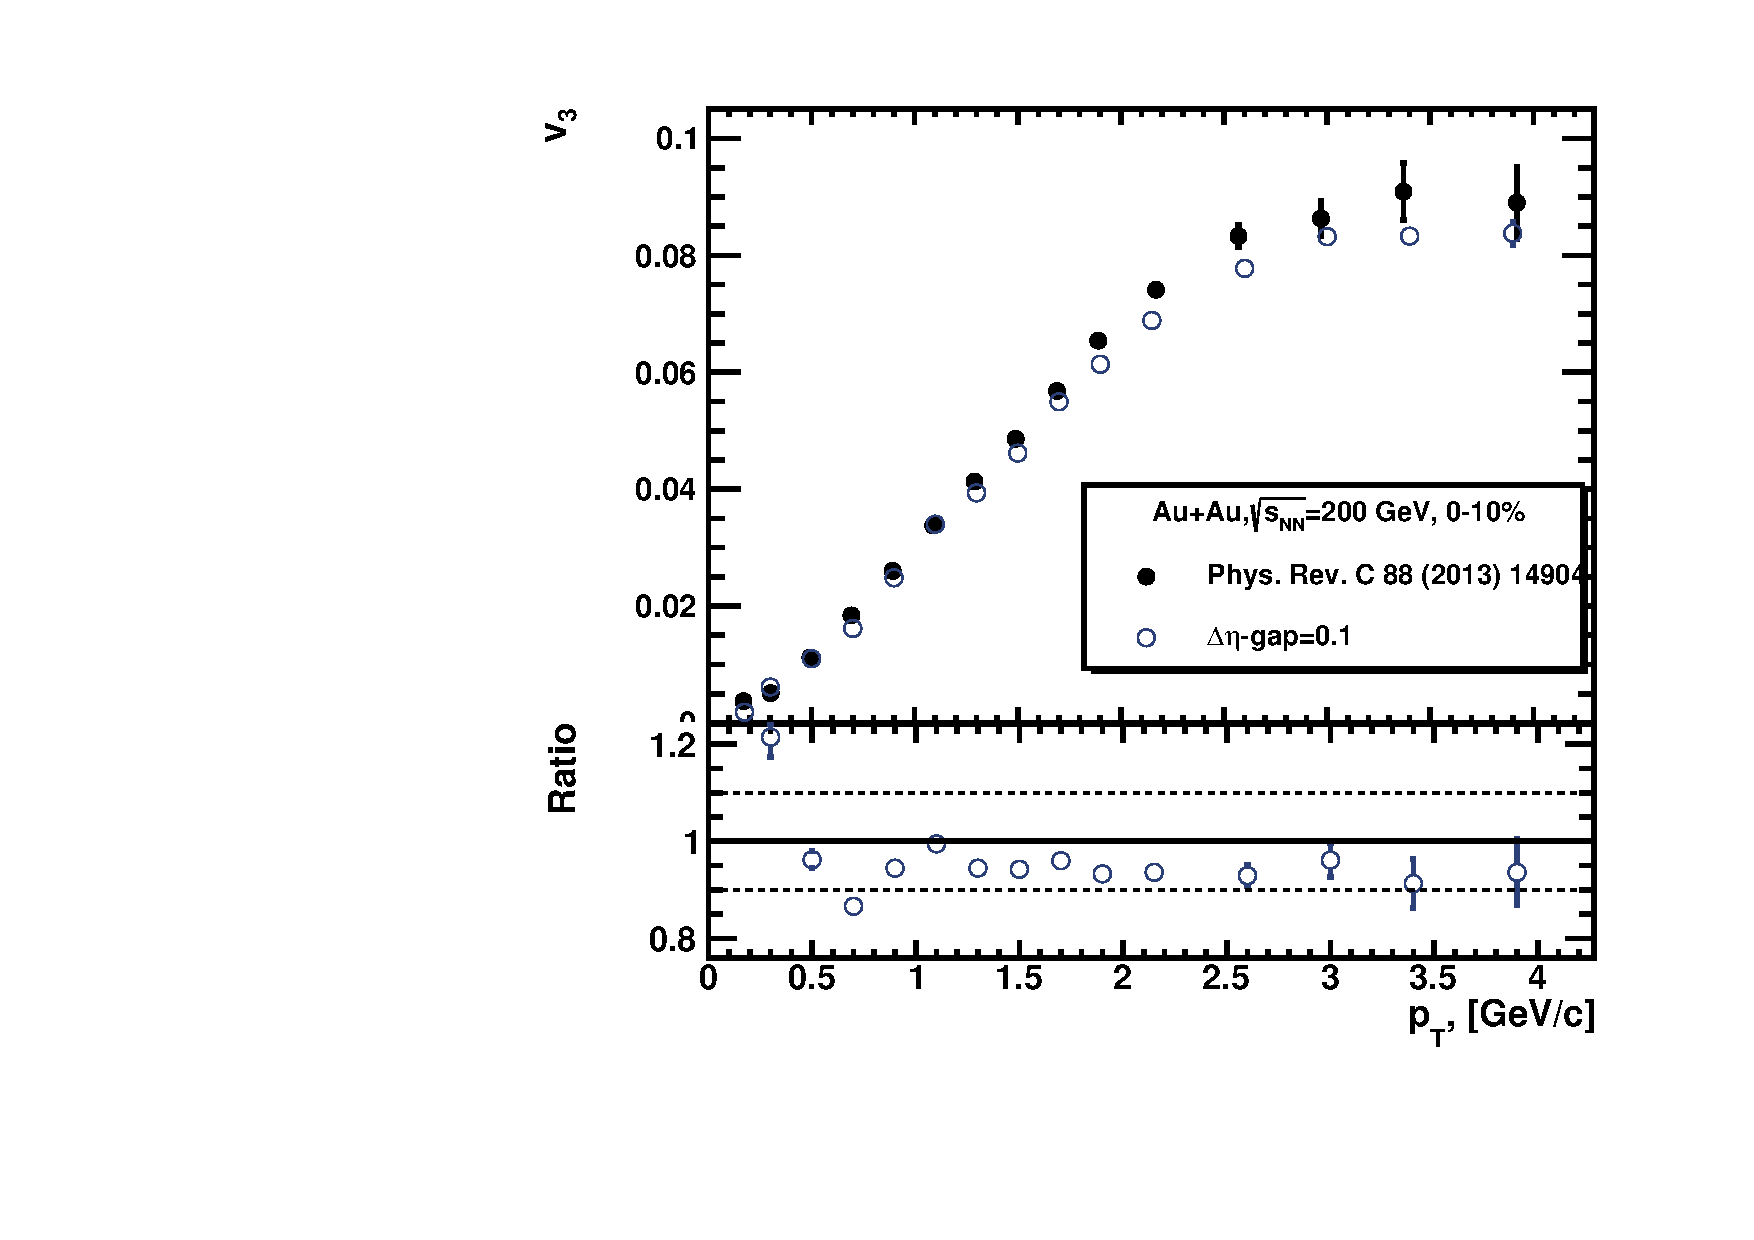
\includegraphics[width=1.\linewidth]{Figures/v3_charged_hadrons_pt_cent0.pdf}
        %\caption{a}
    \end{subfigure}
    \begin{subfigure}{.49\textwidth}
        \centering
        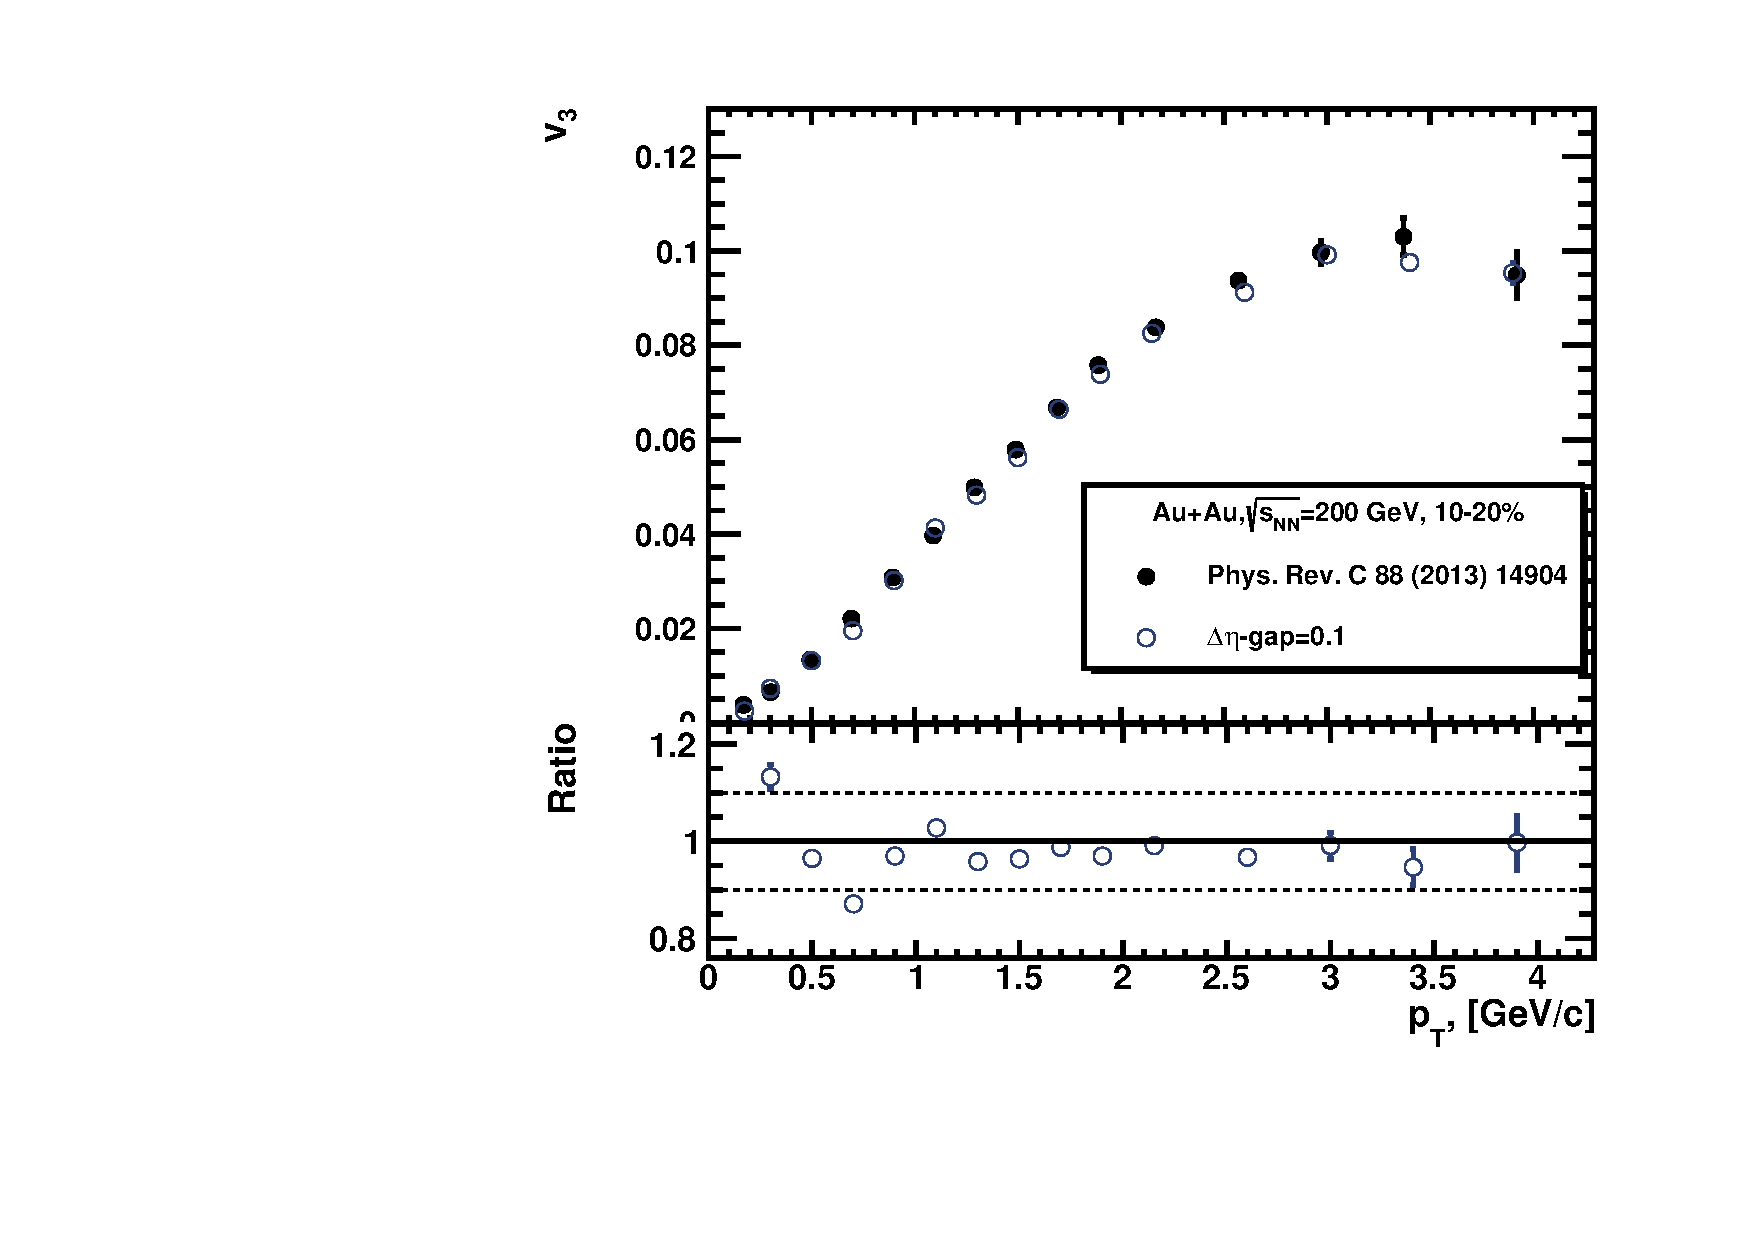
\includegraphics[width=1.\linewidth]{Figures/v3_charged_hadrons_pt_cent1.pdf}
        %\caption{b}
    \end{subfigure}
    \\
    \begin{subfigure}{.49\textwidth}
        \centering
        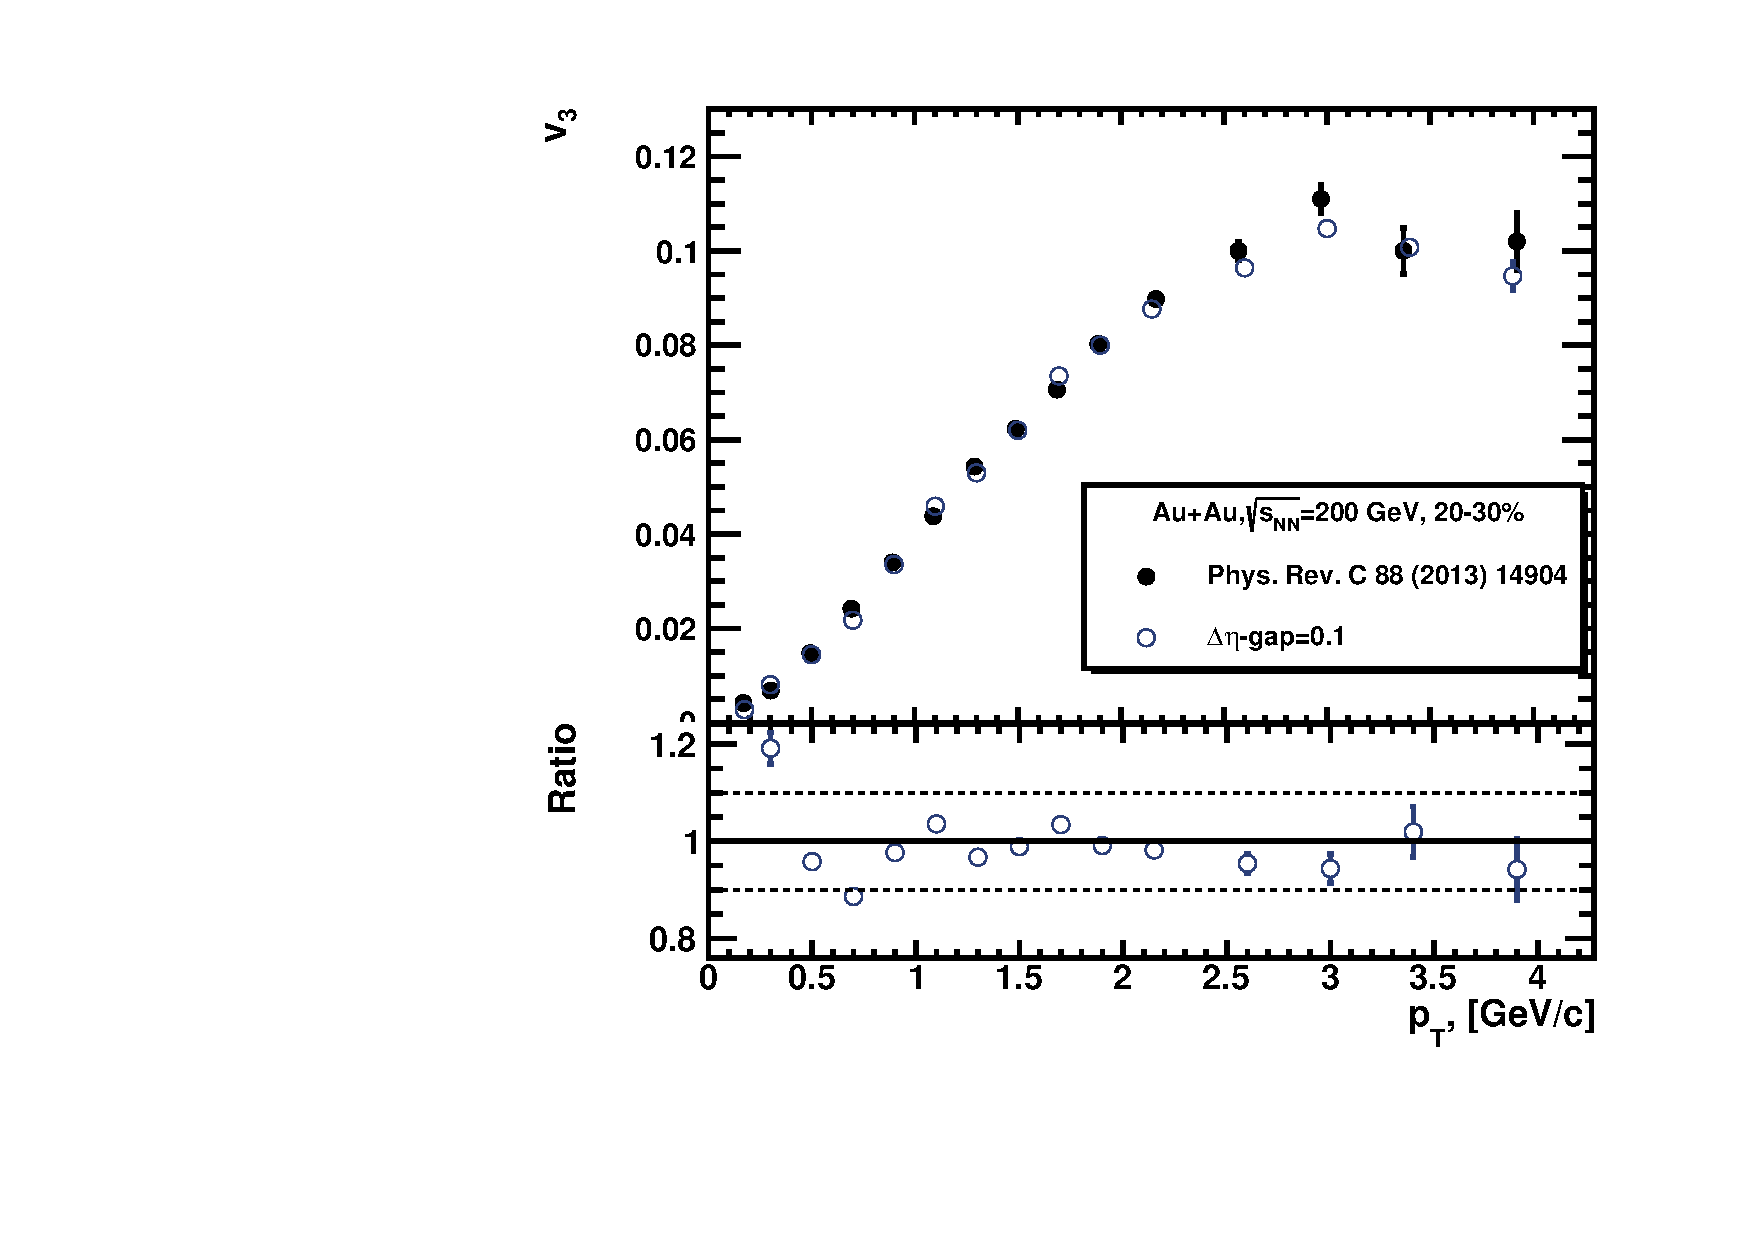
\includegraphics[width=1.\linewidth]{Figures/v3_charged_hadrons_pt_cent2.pdf}
        %\caption{a}
    \end{subfigure}
    \begin{subfigure}{.49\textwidth}
        \centering
        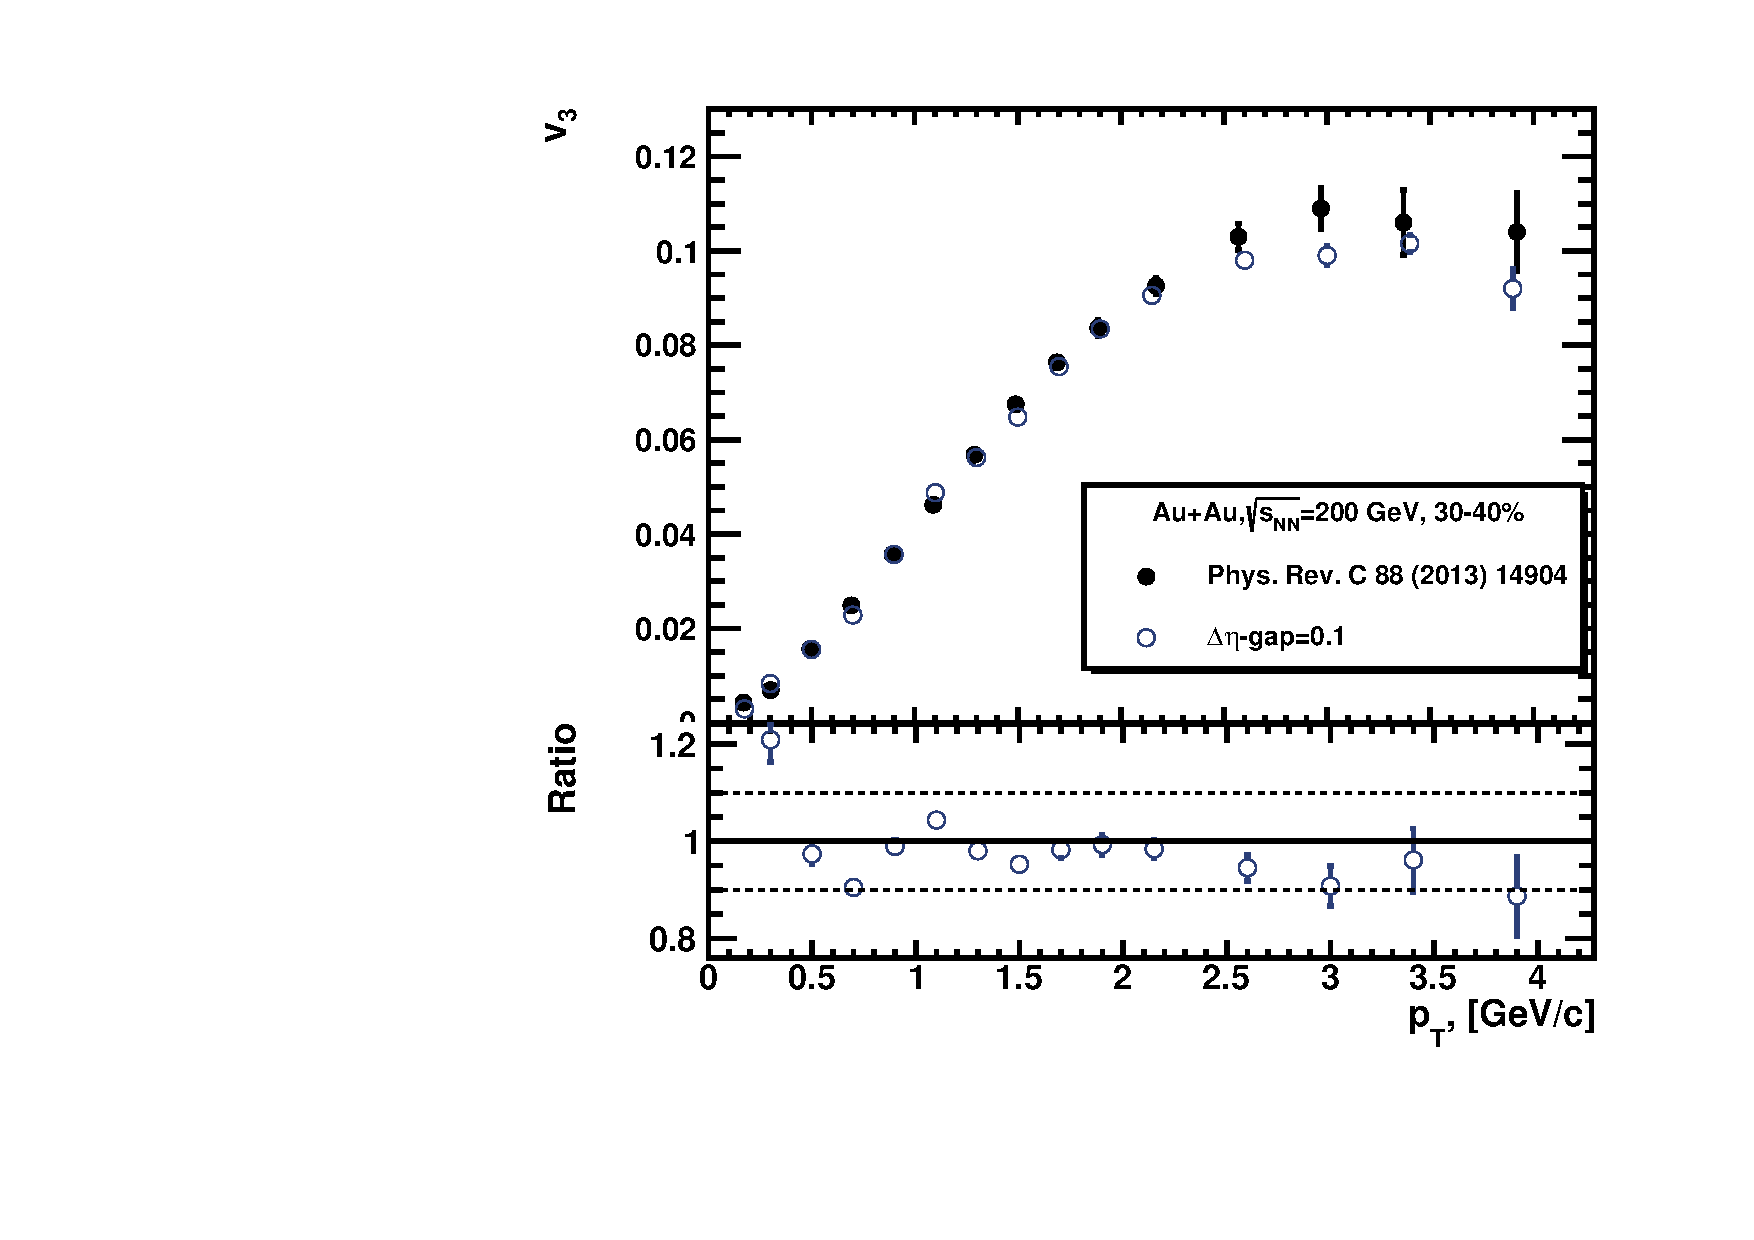
\includegraphics[width=1.\linewidth]{Figures/v3_charged_hadrons_pt_cent3.pdf}
        %\caption{b}
    \end{subfigure}
    \label{fig:v3_EP_CH}
    \caption{Charged hadron $v_3(p_T)$ for 0-10\% (upper left), 10-20\% (upper right), 20-30\% (bottom left) and 30-40 \% (bottom right) centrality classes in \AuAu\ collisions at \sNN\ = 200 GeV. Results were compared with published data \cite{Adamczyk:2013waa}.}
\end{figure}

\FloatBarrier
\subsection{Anisotropic flow for the identified hadrons}

\FloatBarrier
\subsubsection{Elliptic flow}

\begin{figure}[ht]
    \begin{subfigure}{.49\textwidth}
        \centering
        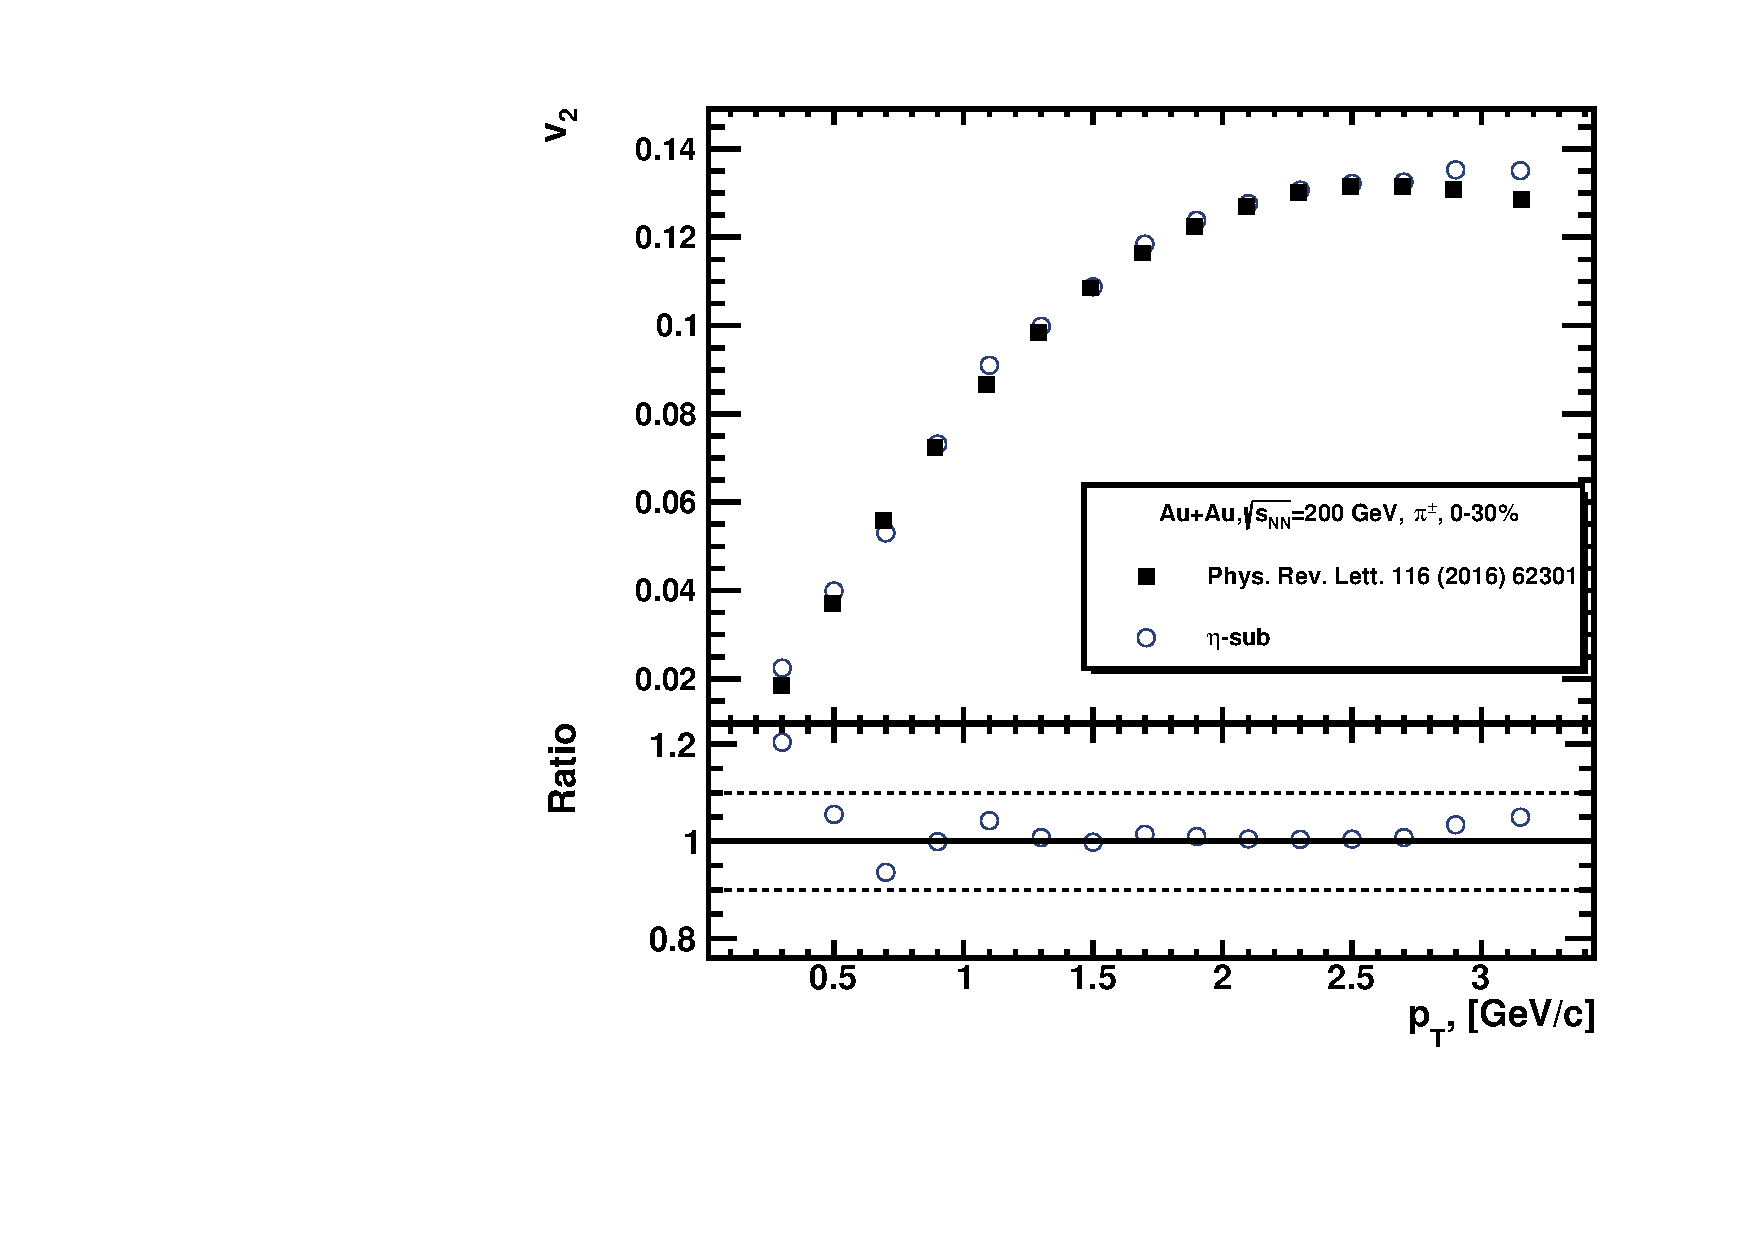
\includegraphics[width=1.\linewidth]{Figures/v2_pions_pt_cent0.pdf}
        %\caption{a}
    \end{subfigure}
    \begin{subfigure}{.49\textwidth}
        \centering
        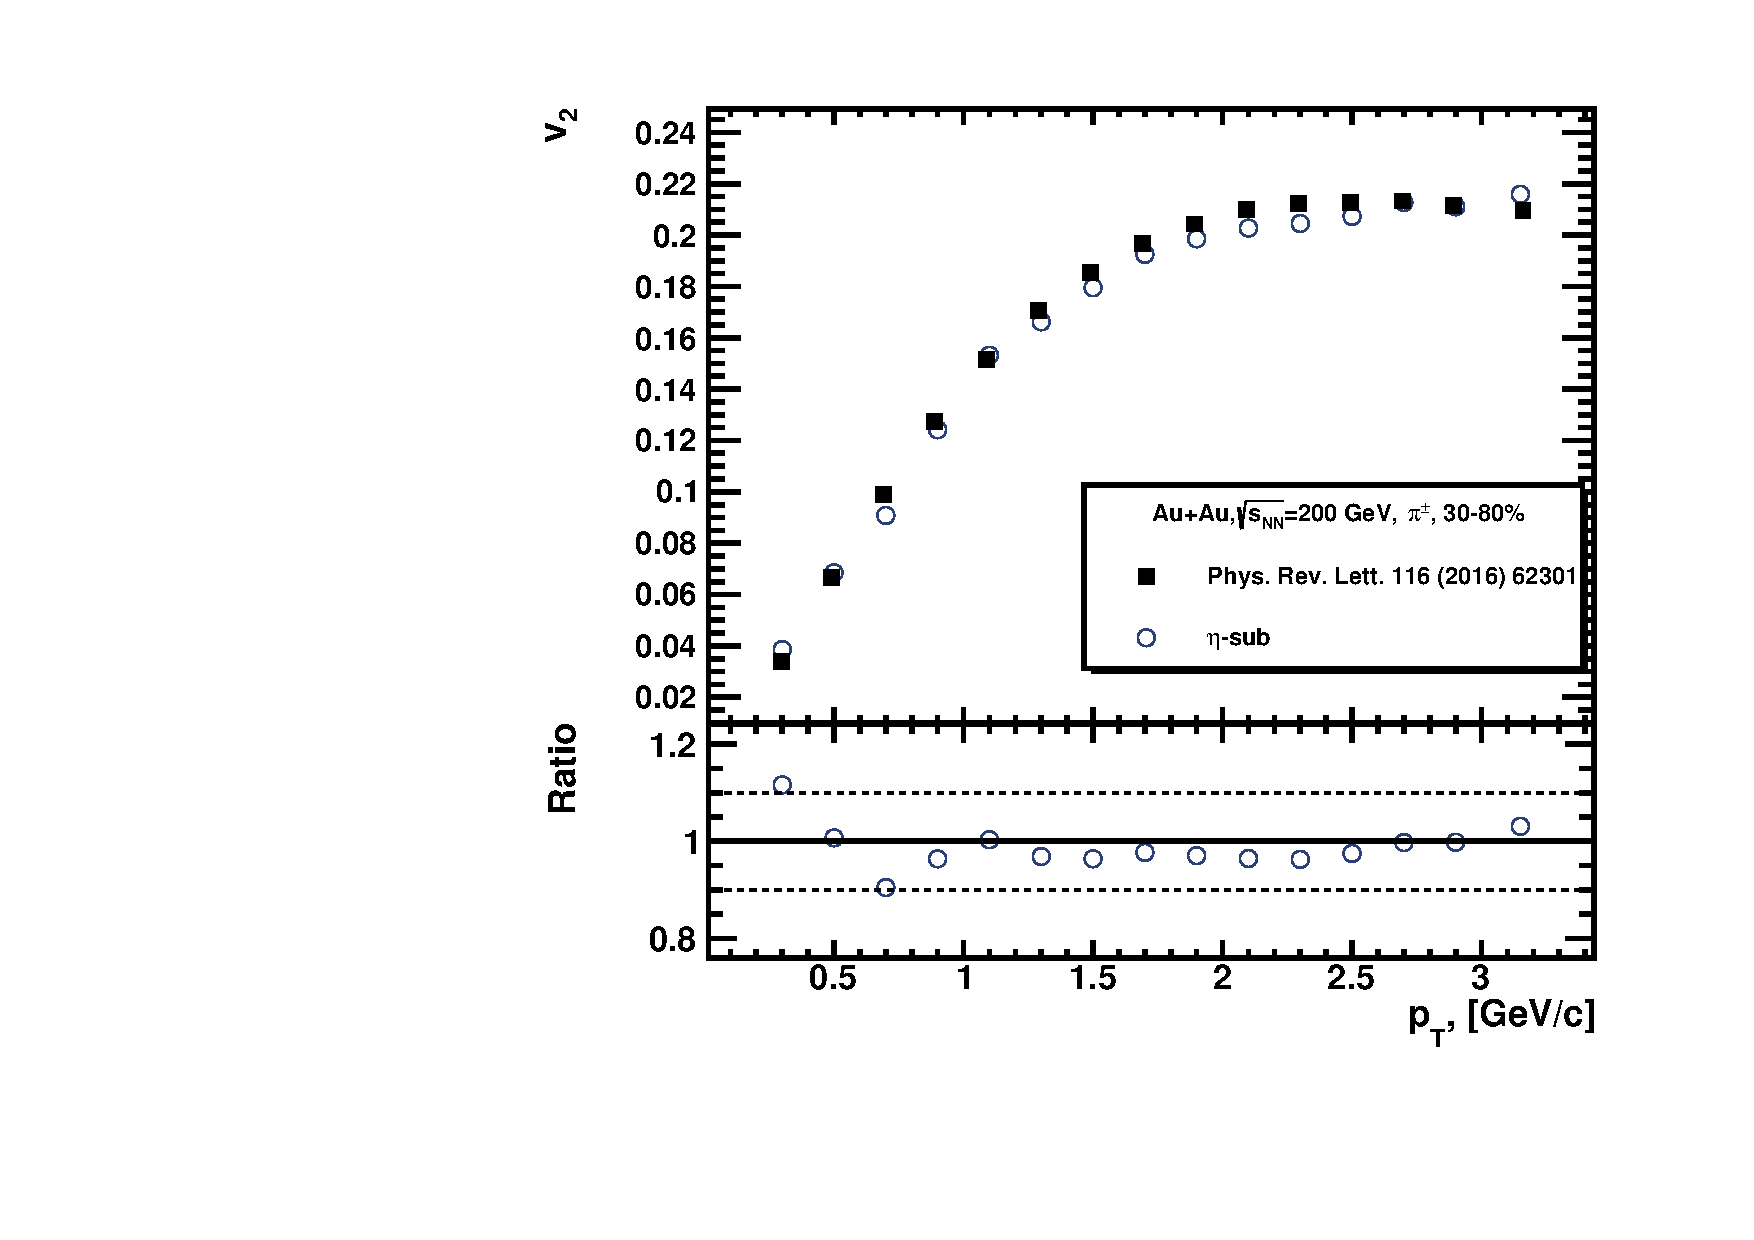
\includegraphics[width=1.\linewidth]{Figures/v2_pions_pt_cent1.pdf}
        %\caption{b}
    \end{subfigure}
    \label{fig:v2_EP_Pions}
    \caption{Pions $v_2(p_T)$ for 0-30\% (left) and 30-80 \% (right) centrality classes in \AuAu\ collisions at \sNN\ = 200 GeV. Results were compared with published data \cite{Adamczyk:2015ukd}.}
\end{figure}

\begin{figure}[ht]
    \begin{subfigure}{.49\textwidth}
        \centering
        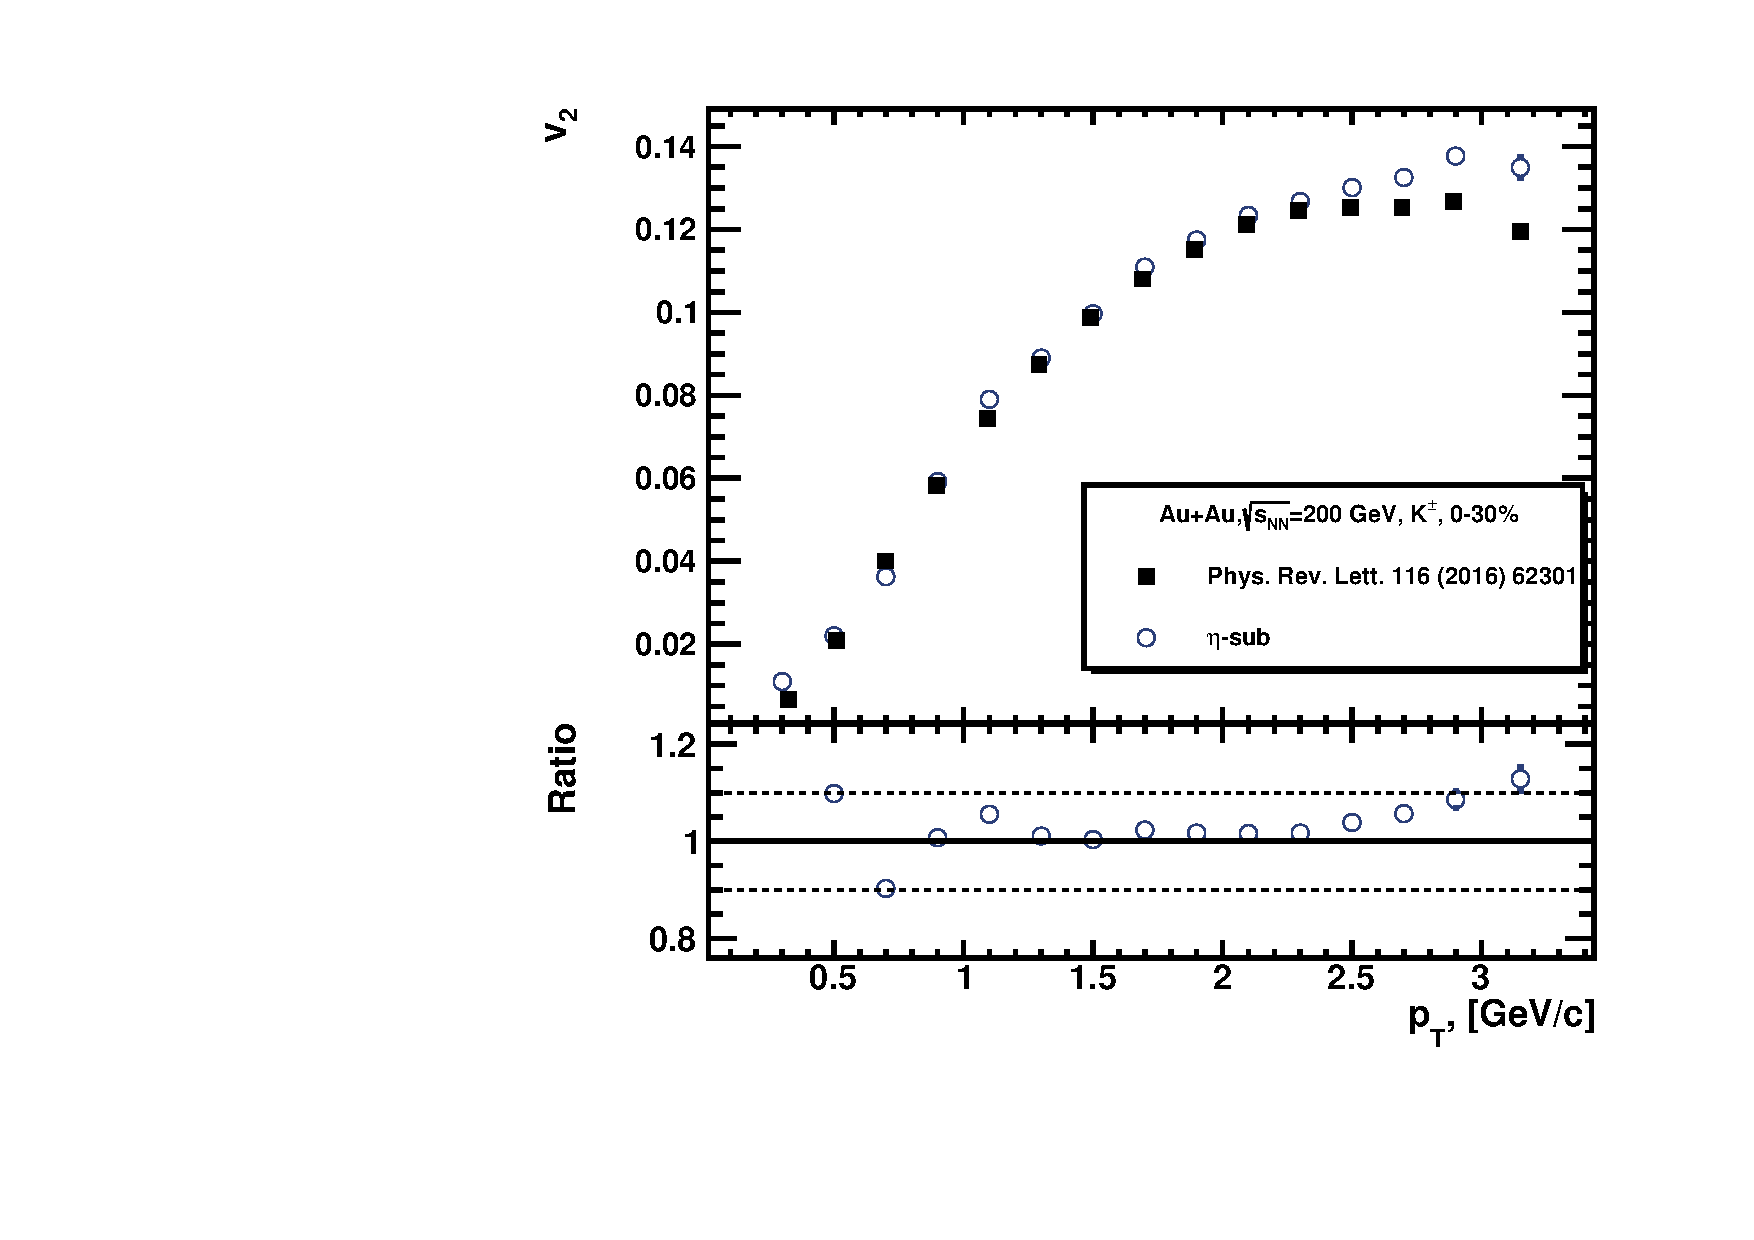
\includegraphics[width=1.\linewidth]{Figures/v2_kaons_pt_cent0.pdf}
        %\caption{a}
    \end{subfigure}
    \begin{subfigure}{.49\textwidth}
        \centering
        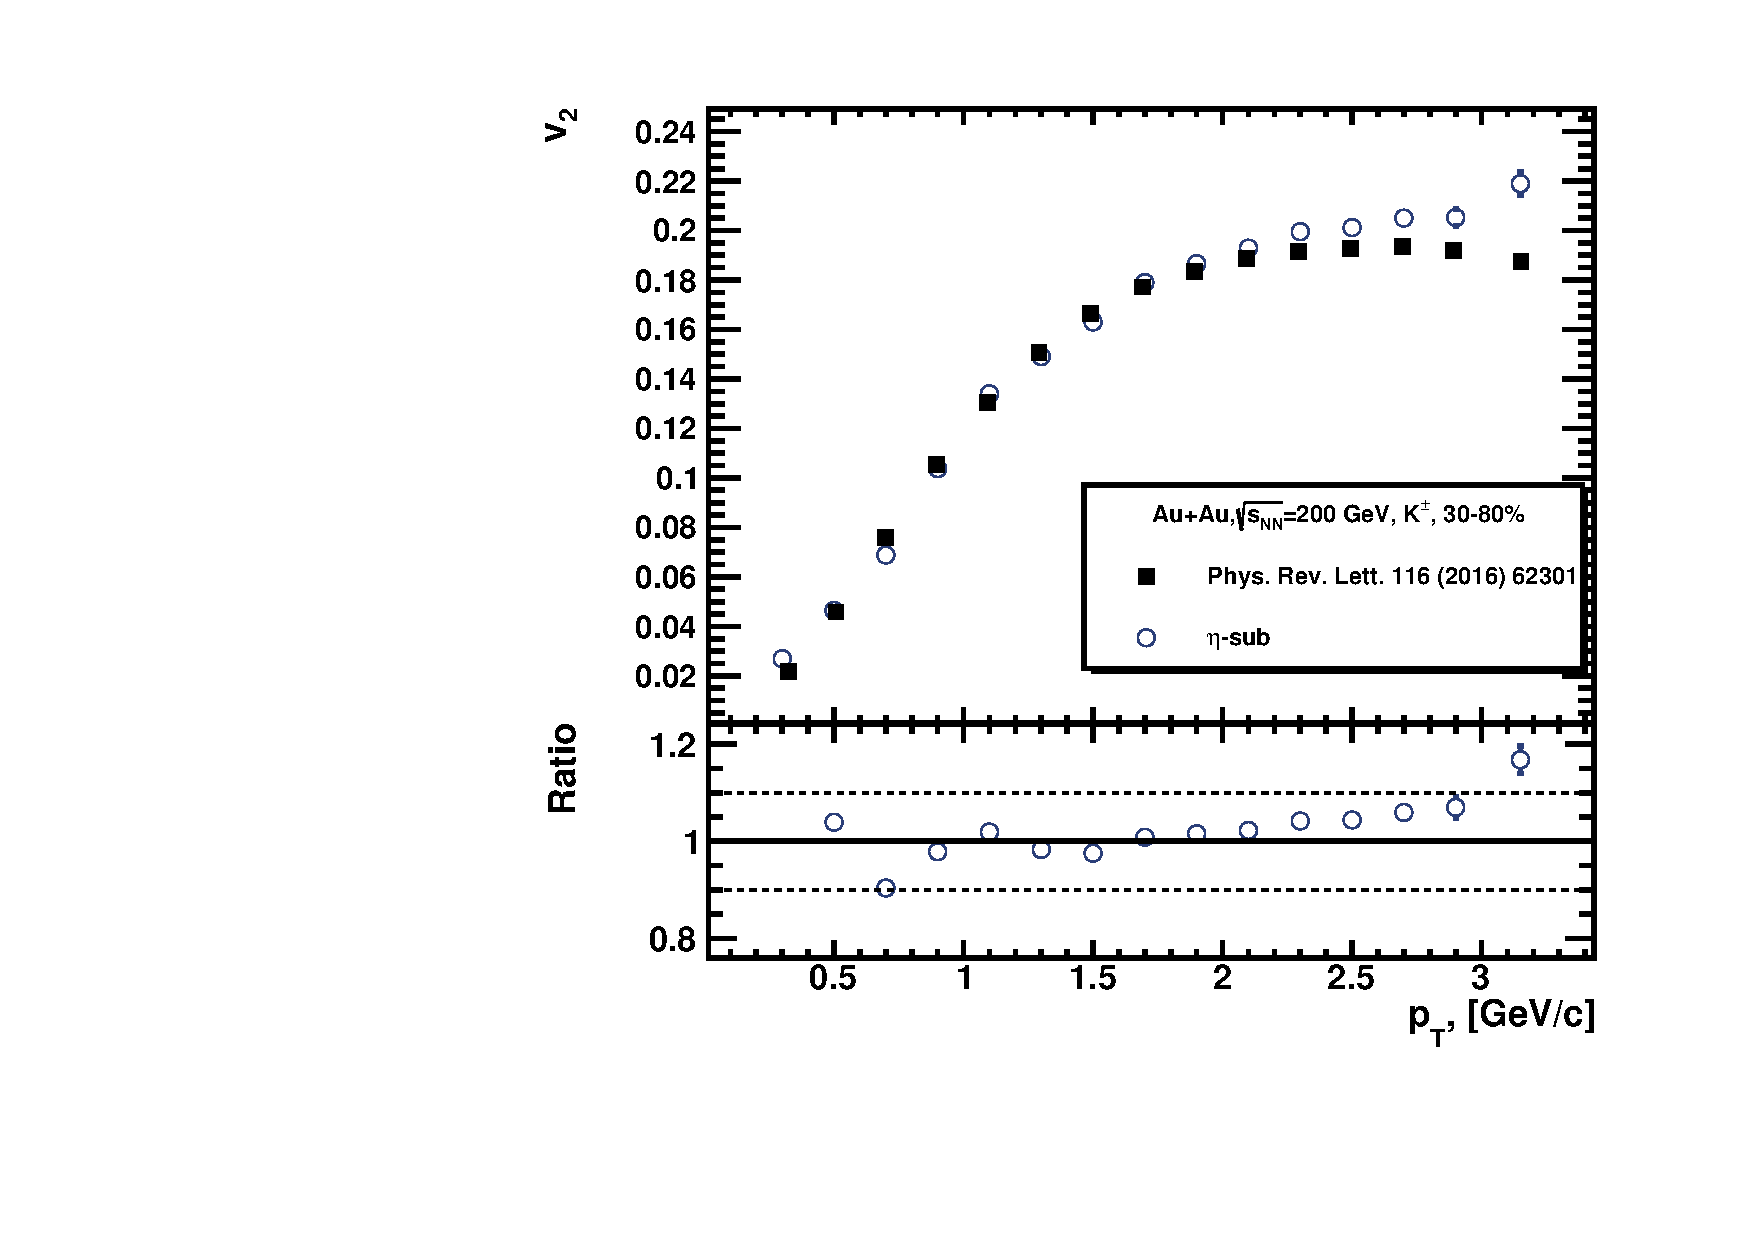
\includegraphics[width=1.\linewidth]{Figures/v2_kaons_pt_cent1.pdf}
        %\caption{b}
    \end{subfigure}
    \label{fig:v2_EP_Kaons}
    \caption{Kaons $v_2(p_T)$ for 0-30\% (left) and 30-80 \% (right) centrality classes in \AuAu\ collisions at \sNN\ = 200 GeV. Results were compared with published data \cite{Adamczyk:2015ukd}.}
\end{figure}

\begin{figure}[ht]
    \begin{subfigure}{.49\textwidth}
        \centering
        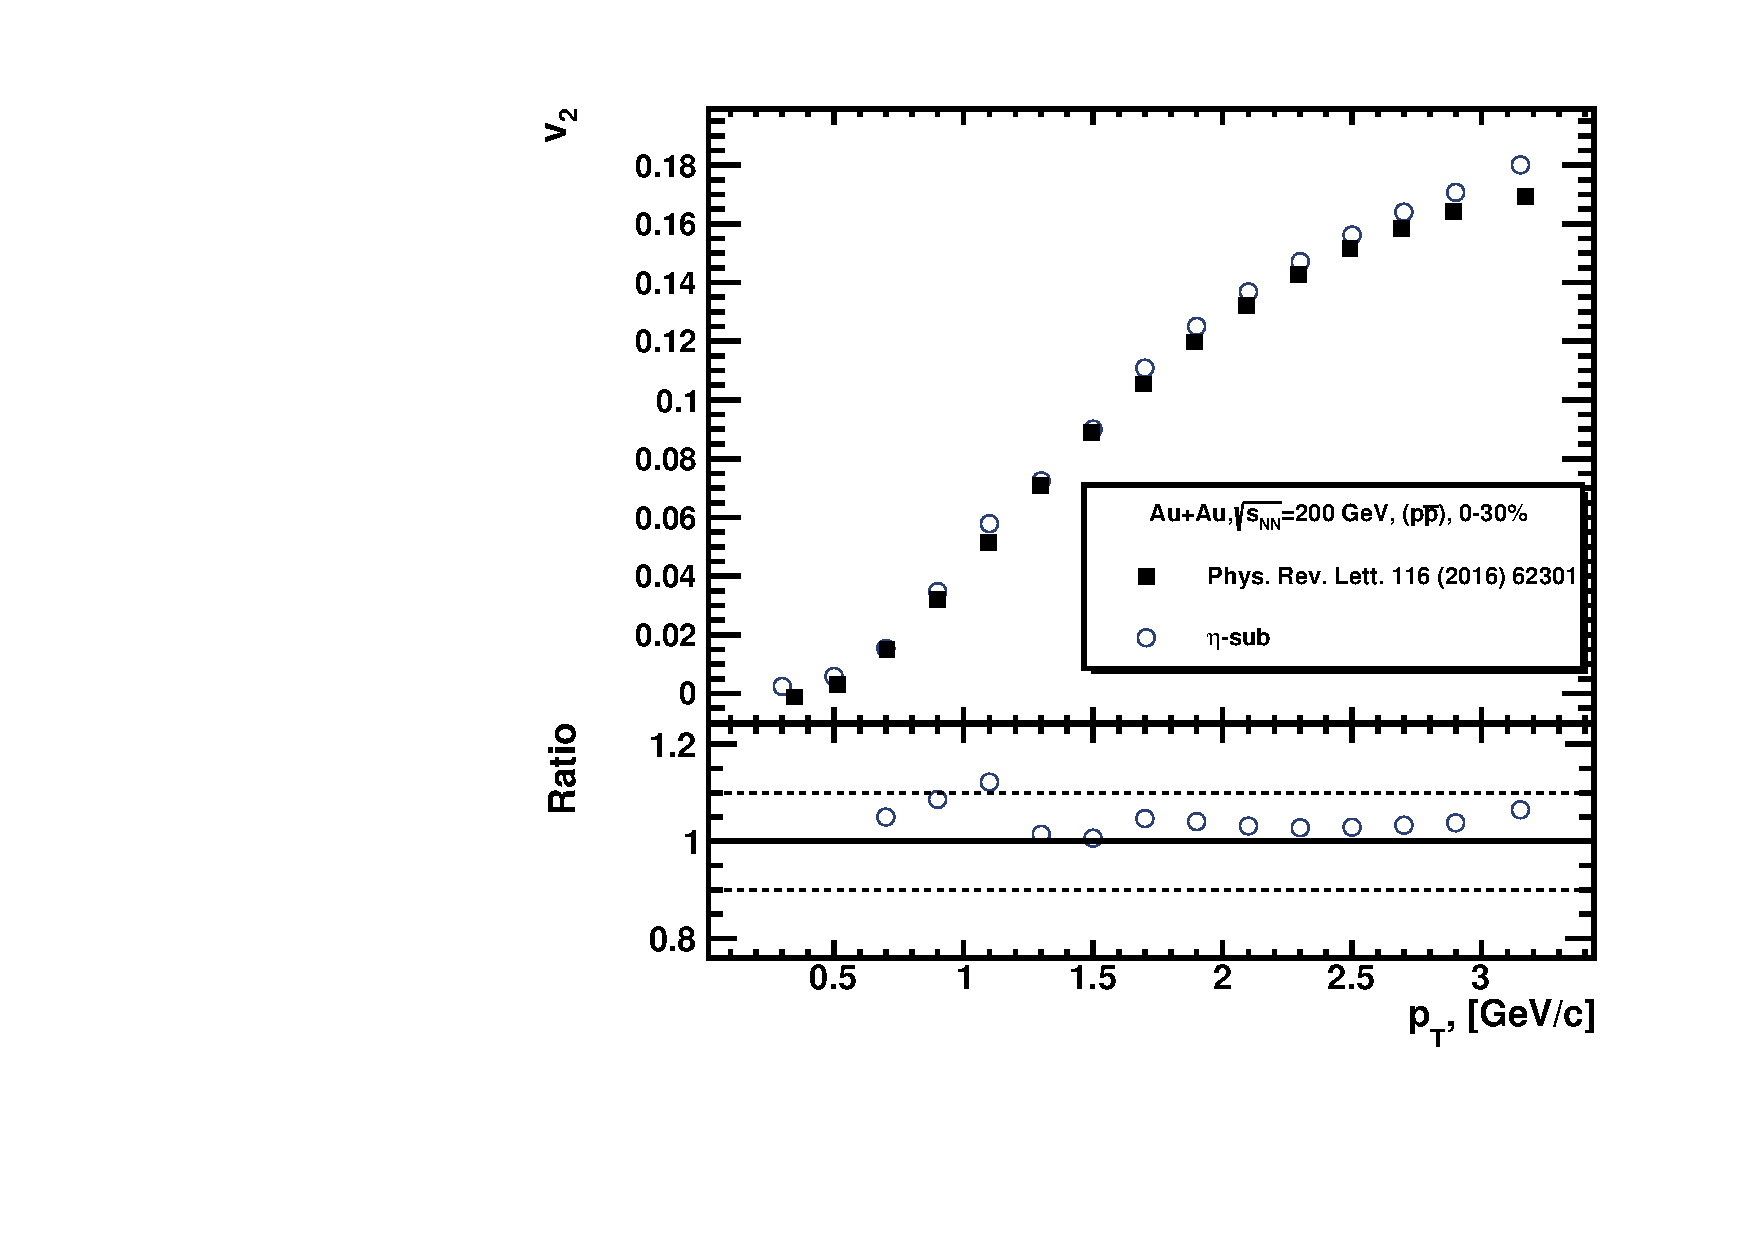
\includegraphics[width=1.\linewidth]{Figures/v2_protons_pt_cent0.pdf}
        %\caption{a}
    \end{subfigure}
    \begin{subfigure}{.49\textwidth}
        \centering
        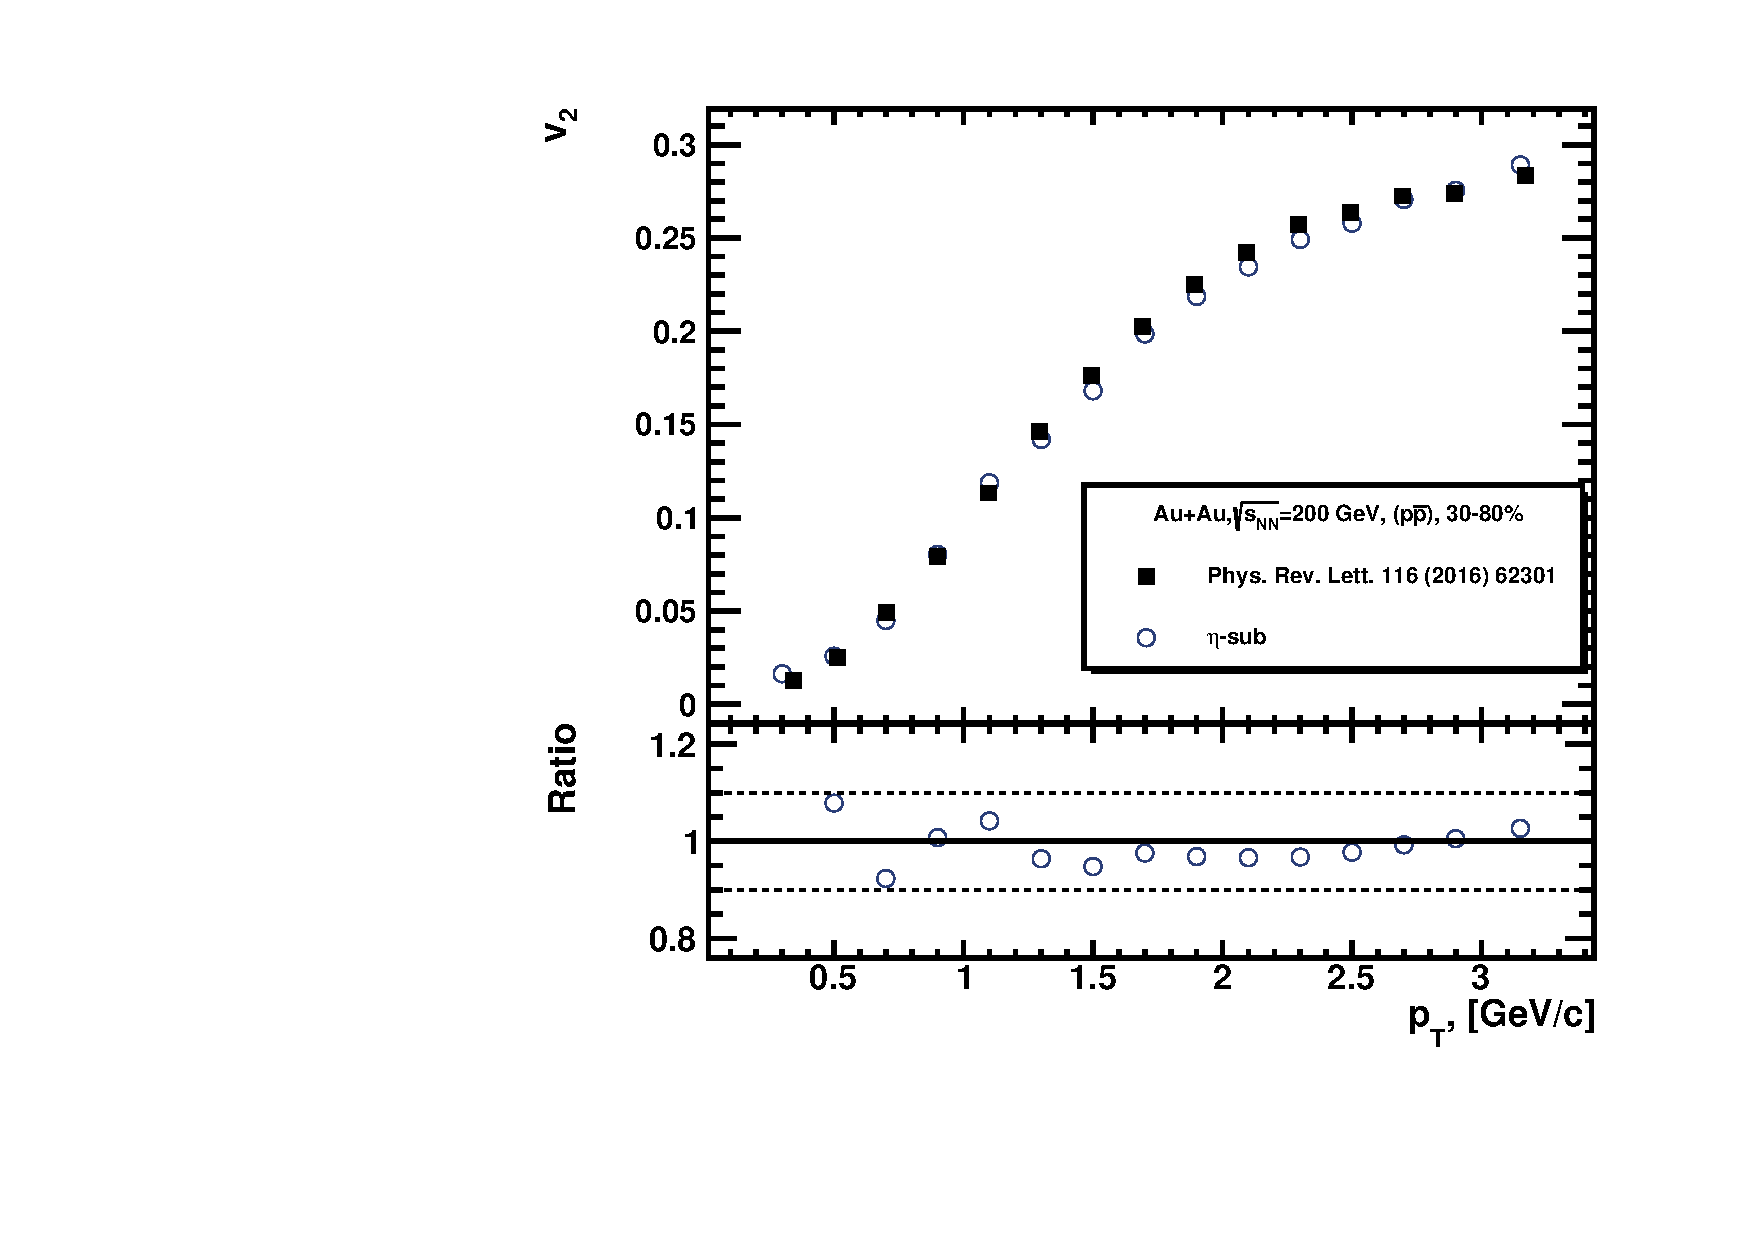
\includegraphics[width=1.\linewidth]{Figures/v2_protons_pt_cent1.pdf}
        %\caption{b}
    \end{subfigure}
    \label{fig:v2_EP_Protons}
    \caption{Protons $v_2(p_T)$ for 0-30\% (left) and 30-80 \% (right) centrality classes in \AuAu\ collisions at \sNN\ = 200 GeV. Results were compared with published data \cite{Adamczyk:2015ukd}.}
\end{figure}

\FloatBarrier
\subsubsection{Triangular flow}

\begin{figure}[ht]
    \begin{subfigure}{.49\textwidth}
        \centering
        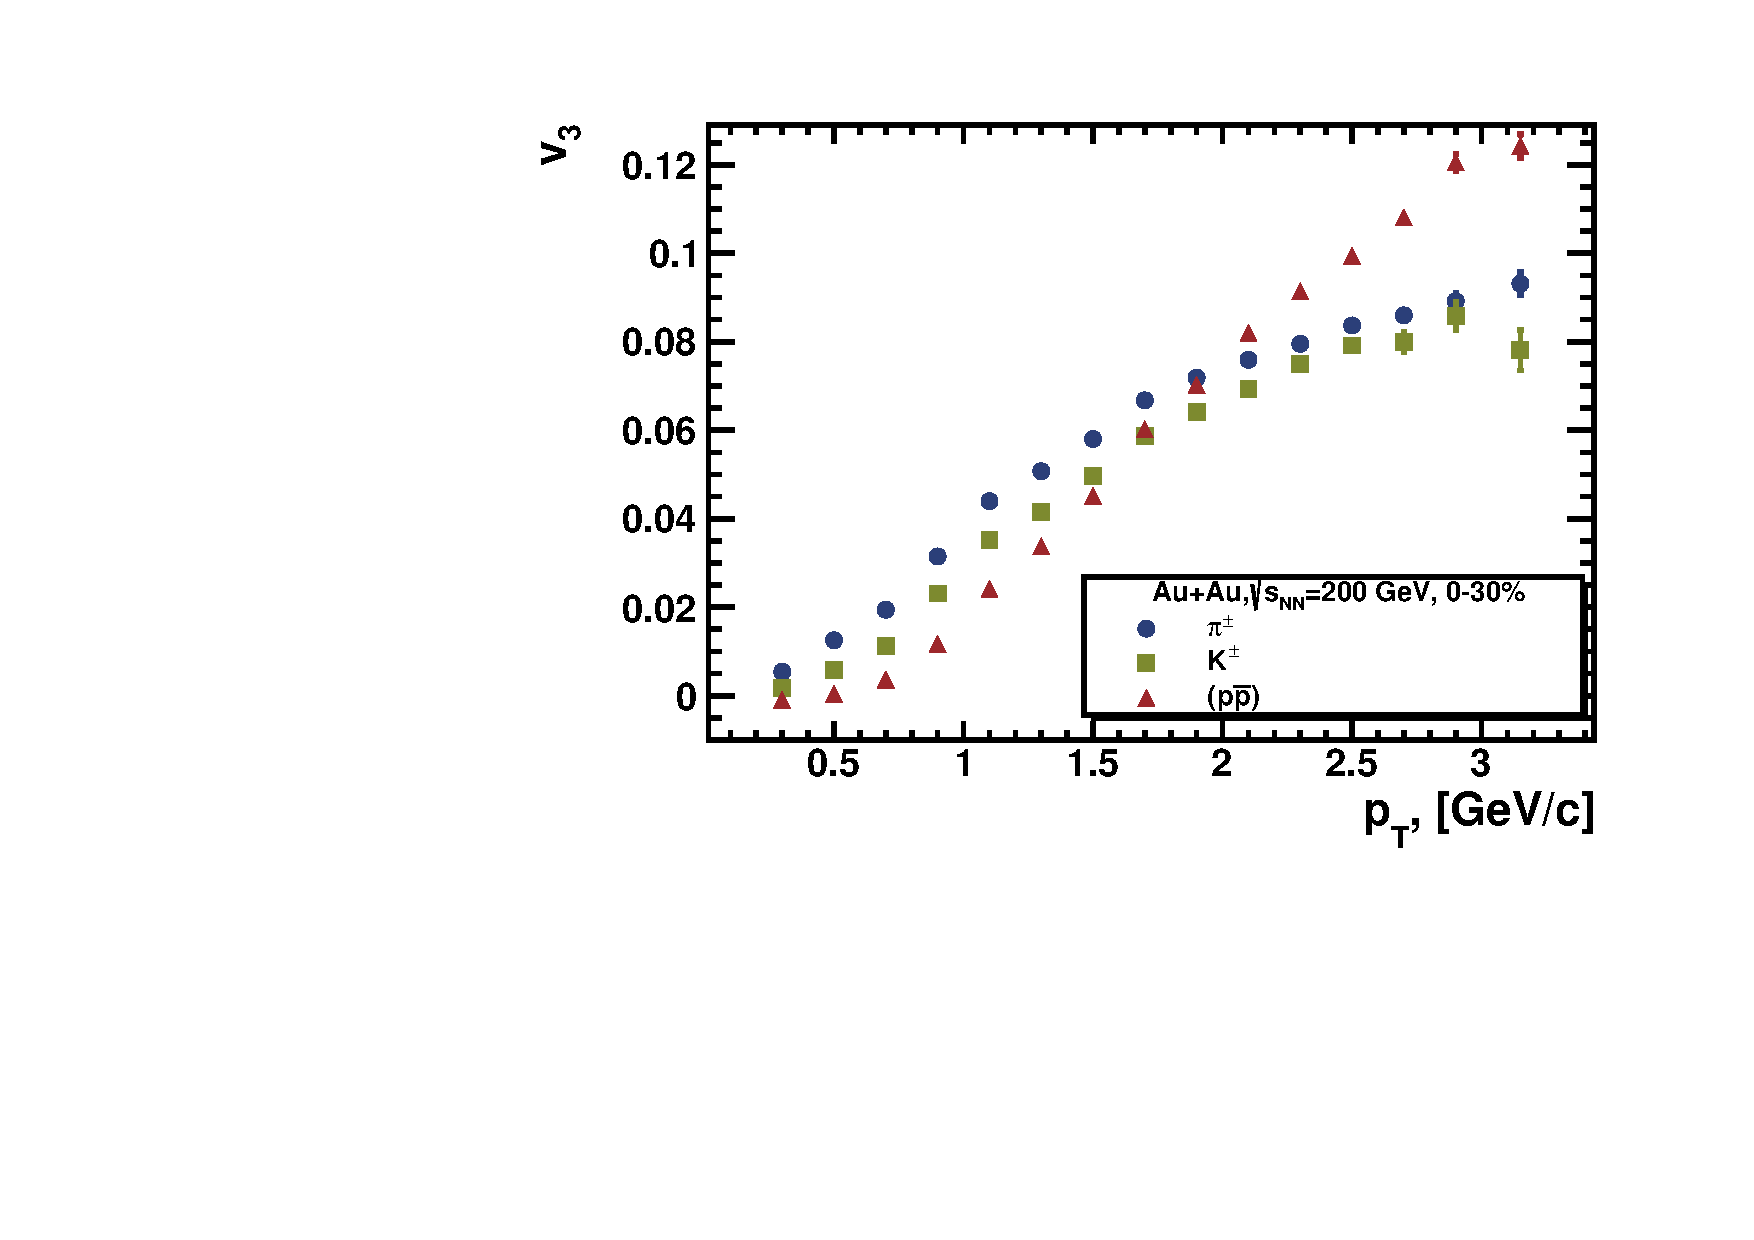
\includegraphics[width=1.\linewidth]{Figures/v3_Total_pt_cent0.pdf}
        %\caption{a}
    \end{subfigure}
    \begin{subfigure}{.49\textwidth}
        \centering
        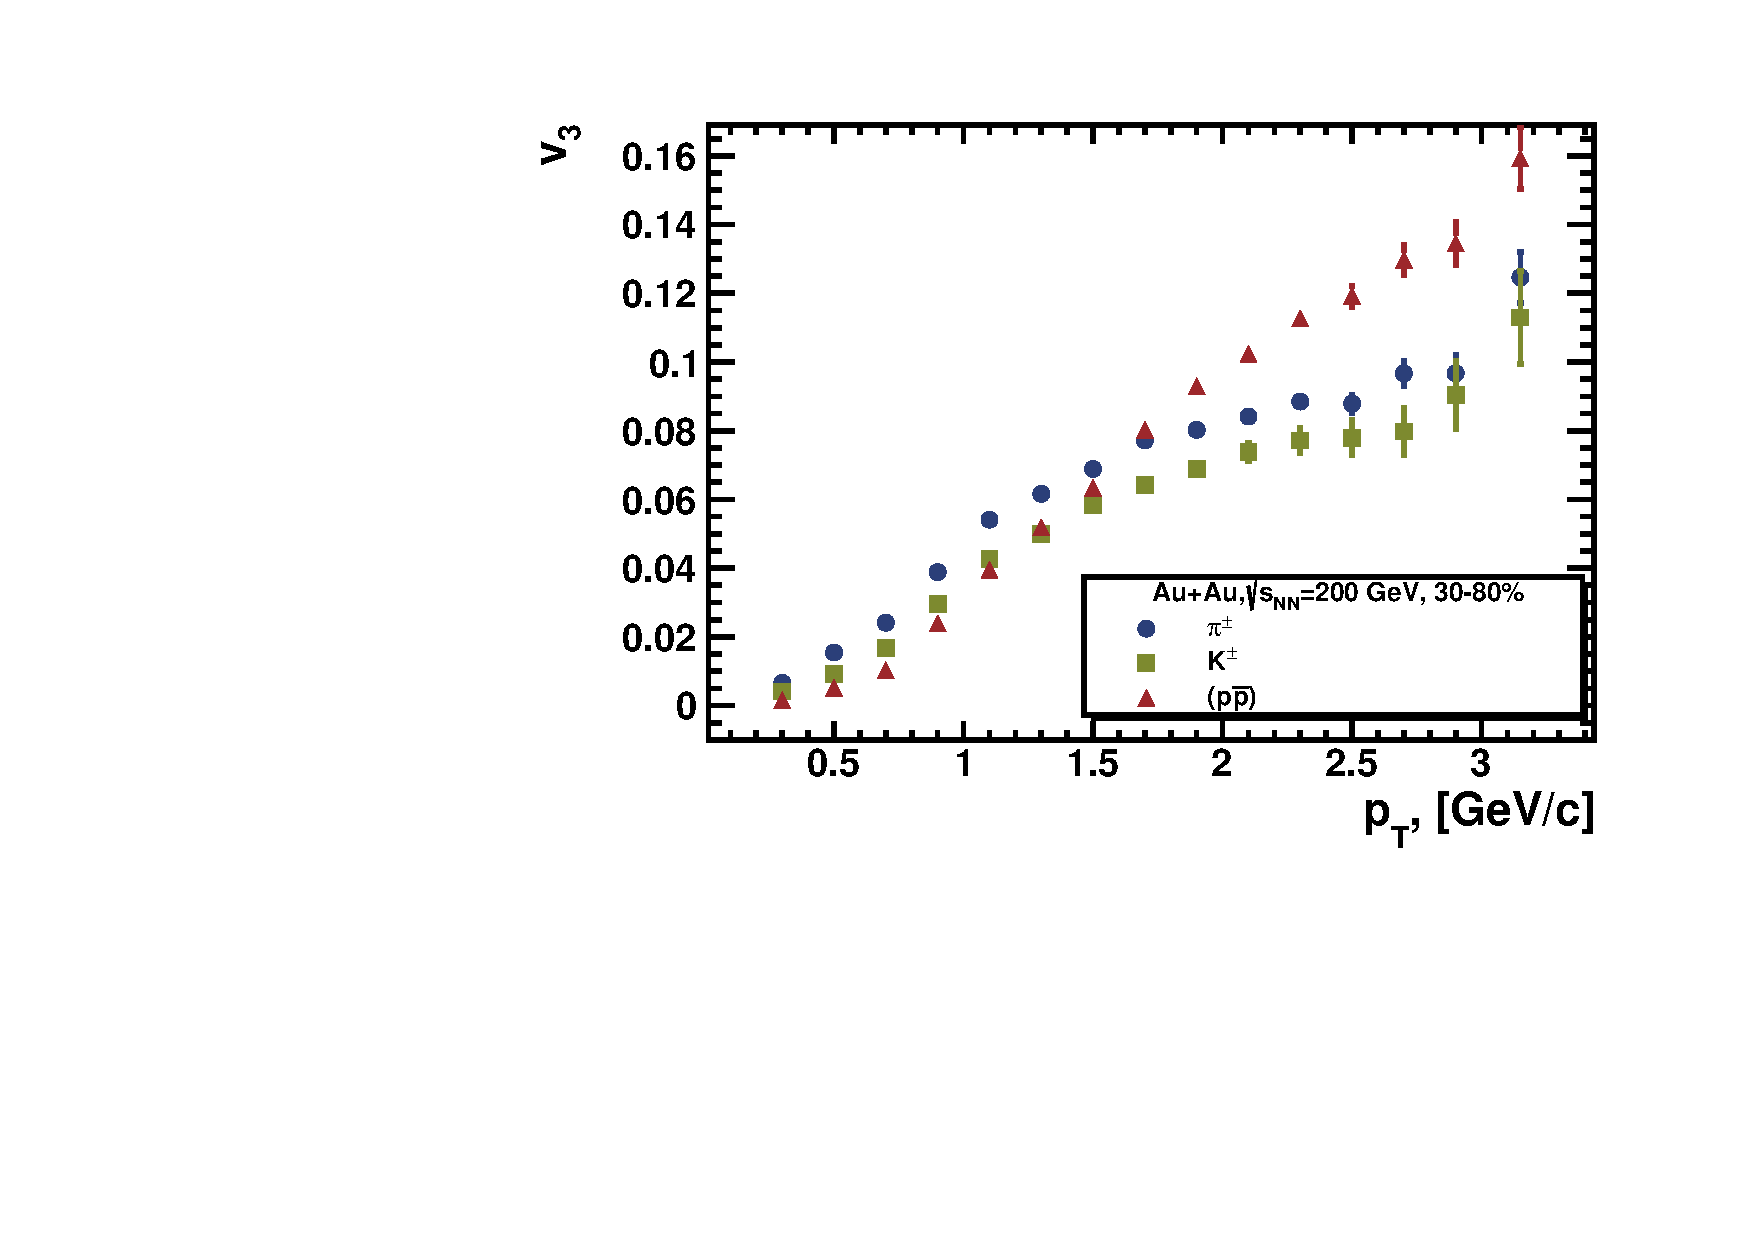
\includegraphics[width=1.\linewidth]{Figures/v3_Total_pt_cent1.pdf}
        %\caption{b}
    \end{subfigure}
    \label{fig:v3_EP_PID}
    \caption{Identified hadrons $v_3(p_T)$ for 0-30\% (left) and 30-80 \% (right) centrality classes in \AuAu\ collisions at \sNN\ = 200 GeV.}
\end{figure}

\FloatBarrier
\subsection{Method comparison}
\FloatBarrier
\subsubsection{Scalar product method}

\begin{figure}[ht]
    \begin{subfigure}{.49\textwidth}
        \centering
        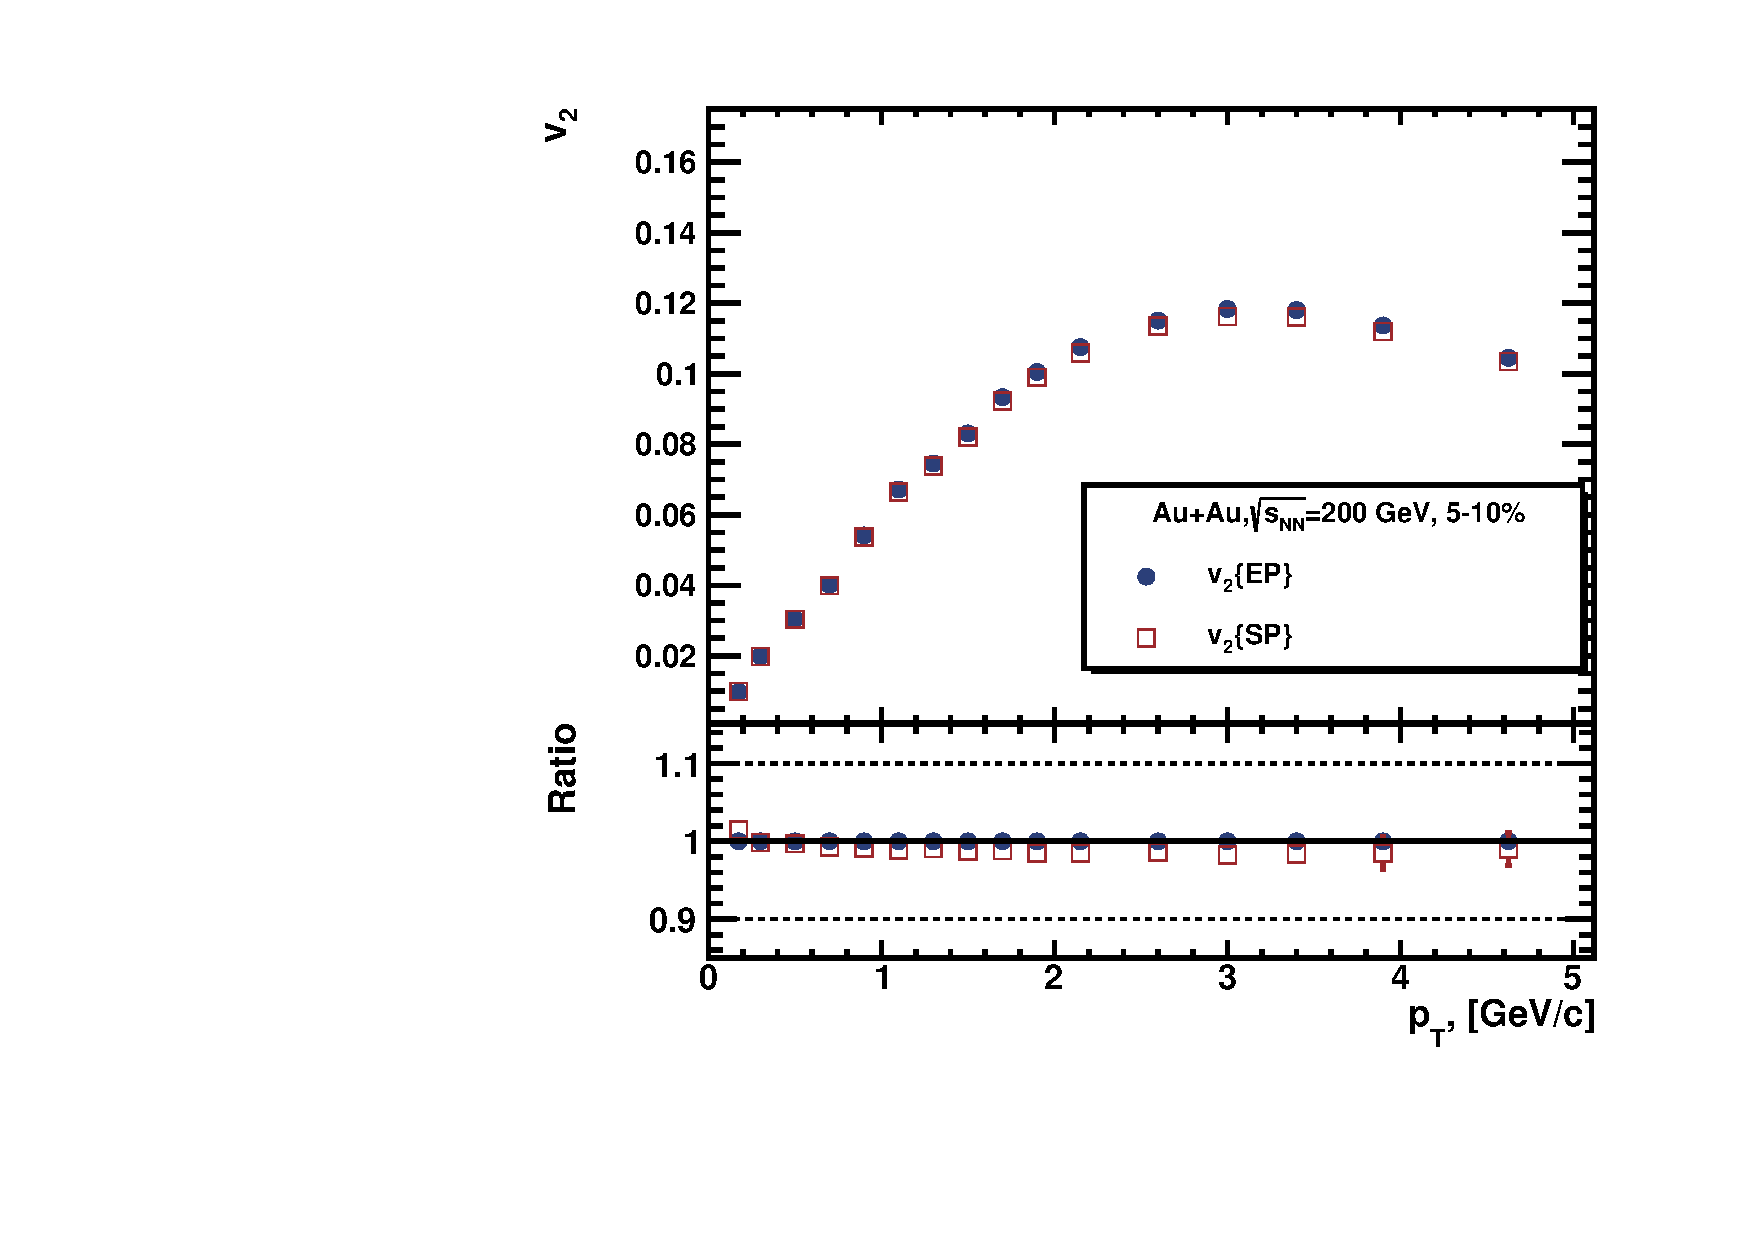
\includegraphics[width=1.\linewidth]{Figures/v2_CH_SP_pt_cent1.pdf}
        %\caption{a}
    \end{subfigure}
    \begin{subfigure}{.49\textwidth}
        \centering
        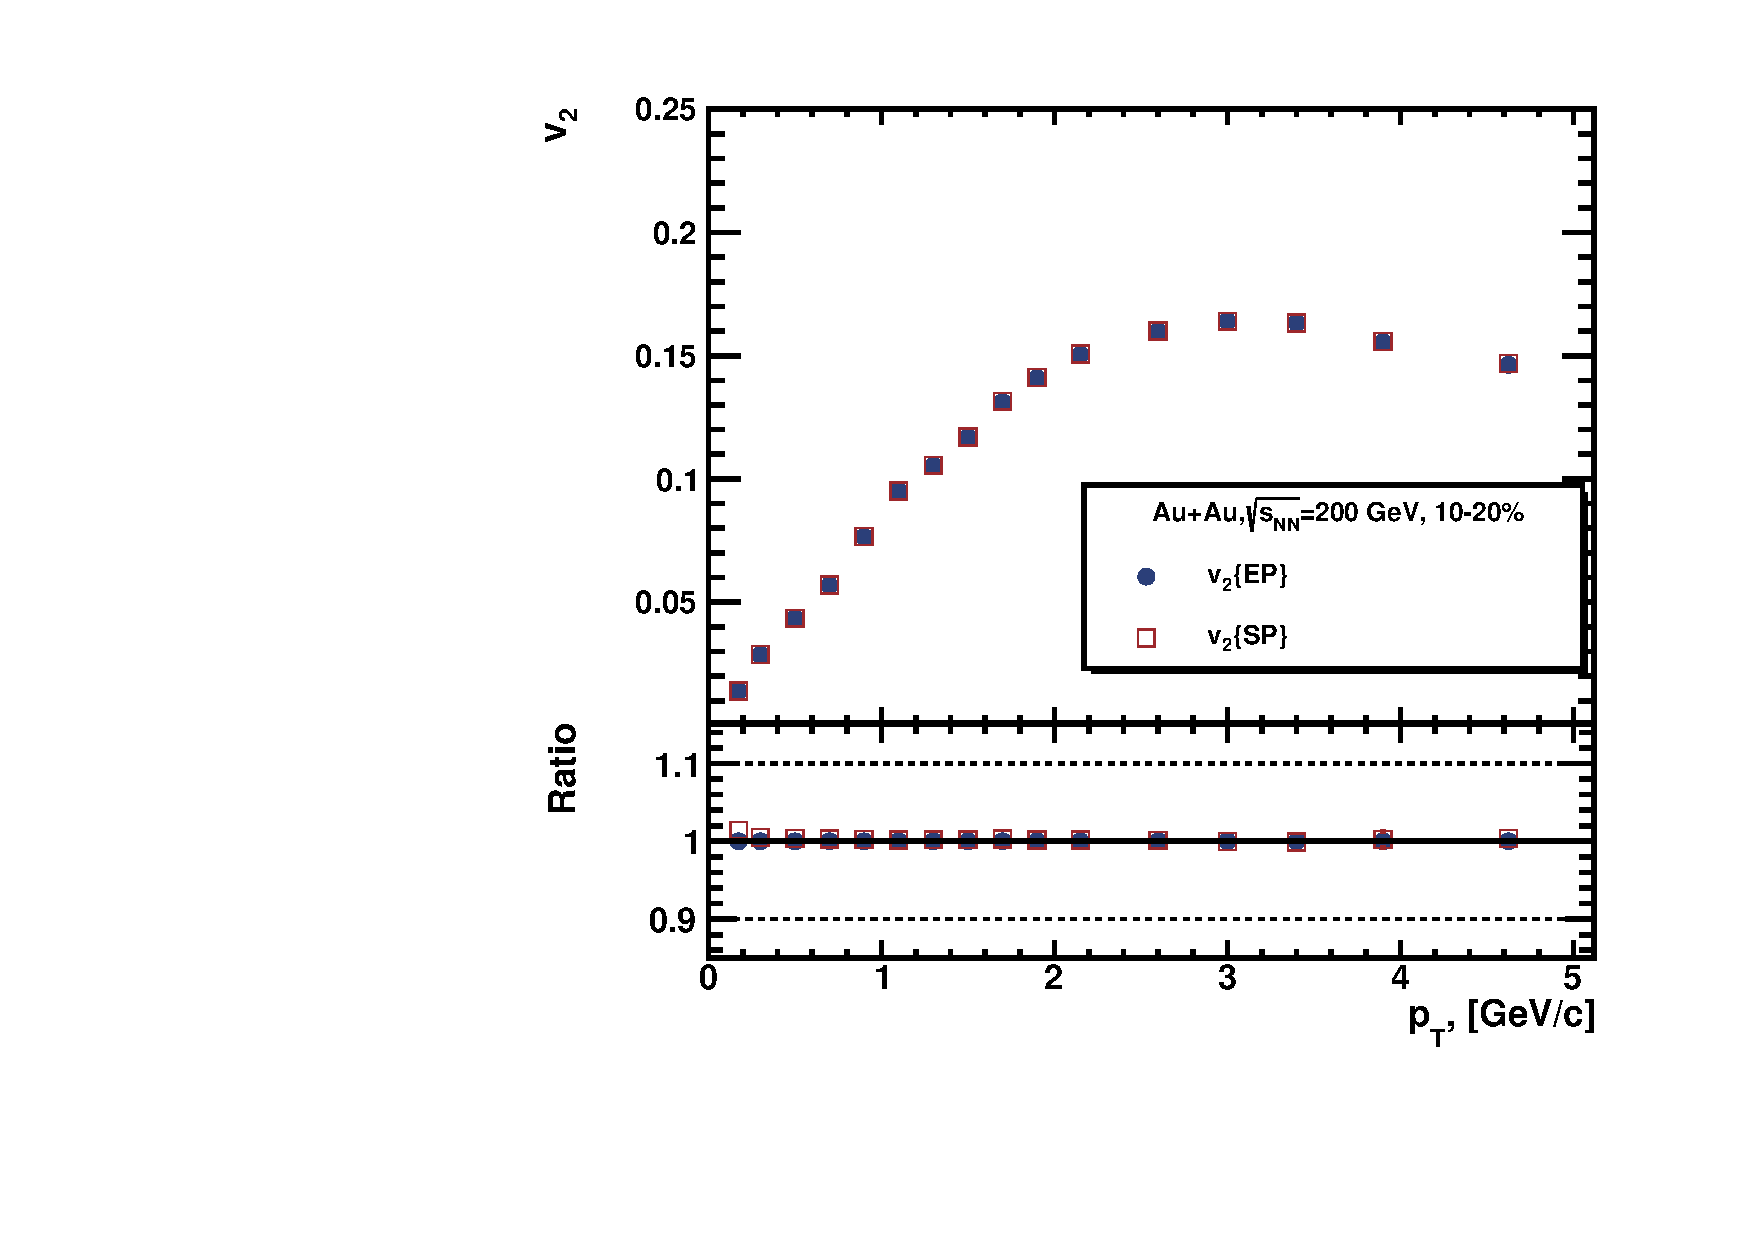
\includegraphics[width=1.\linewidth]{Figures/v2_CH_SP_pt_cent2.pdf}
        %\caption{b}
    \end{subfigure}
    \\
    \begin{subfigure}{.49\textwidth}
        \centering
        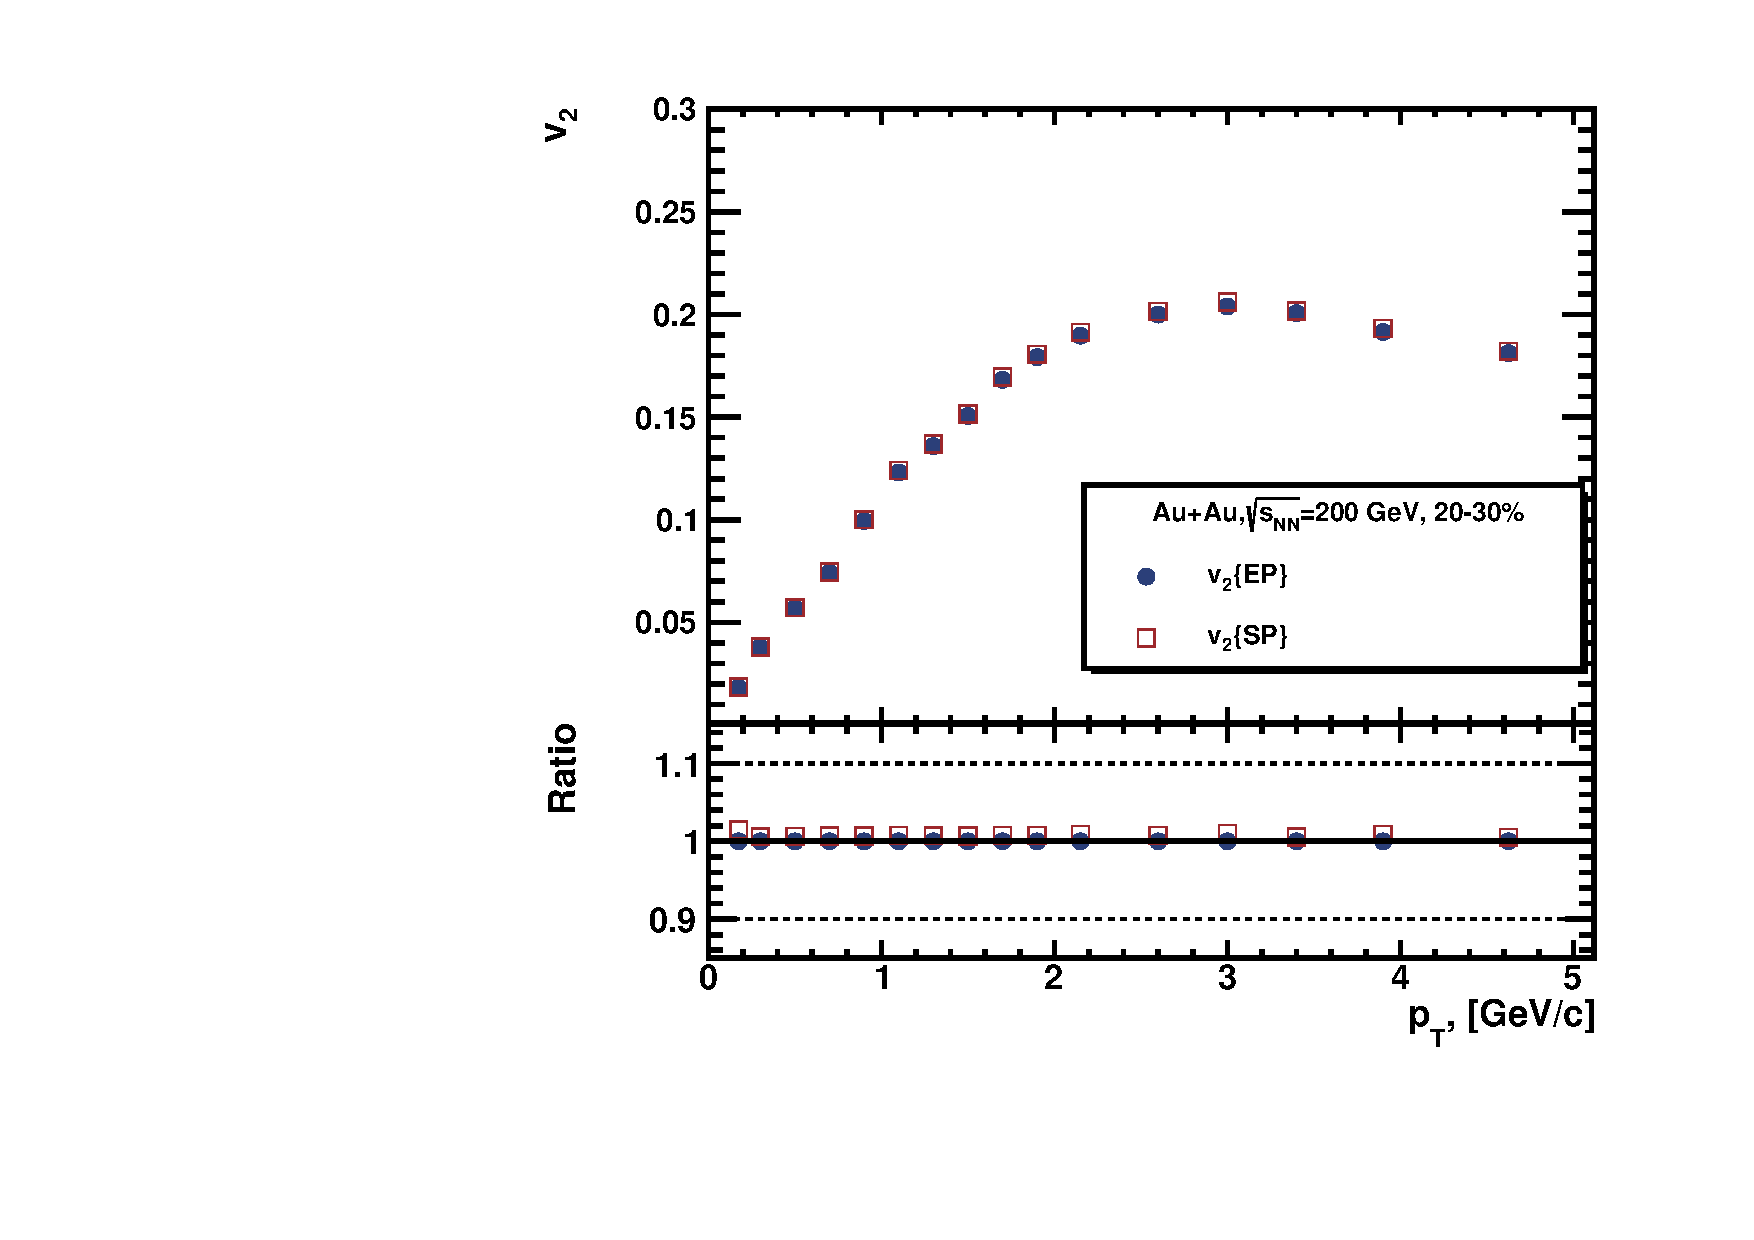
\includegraphics[width=1.\linewidth]{Figures/v2_CH_SP_pt_cent3.pdf}
        %\caption{a}
    \end{subfigure}
    \begin{subfigure}{.49\textwidth}
        \centering
        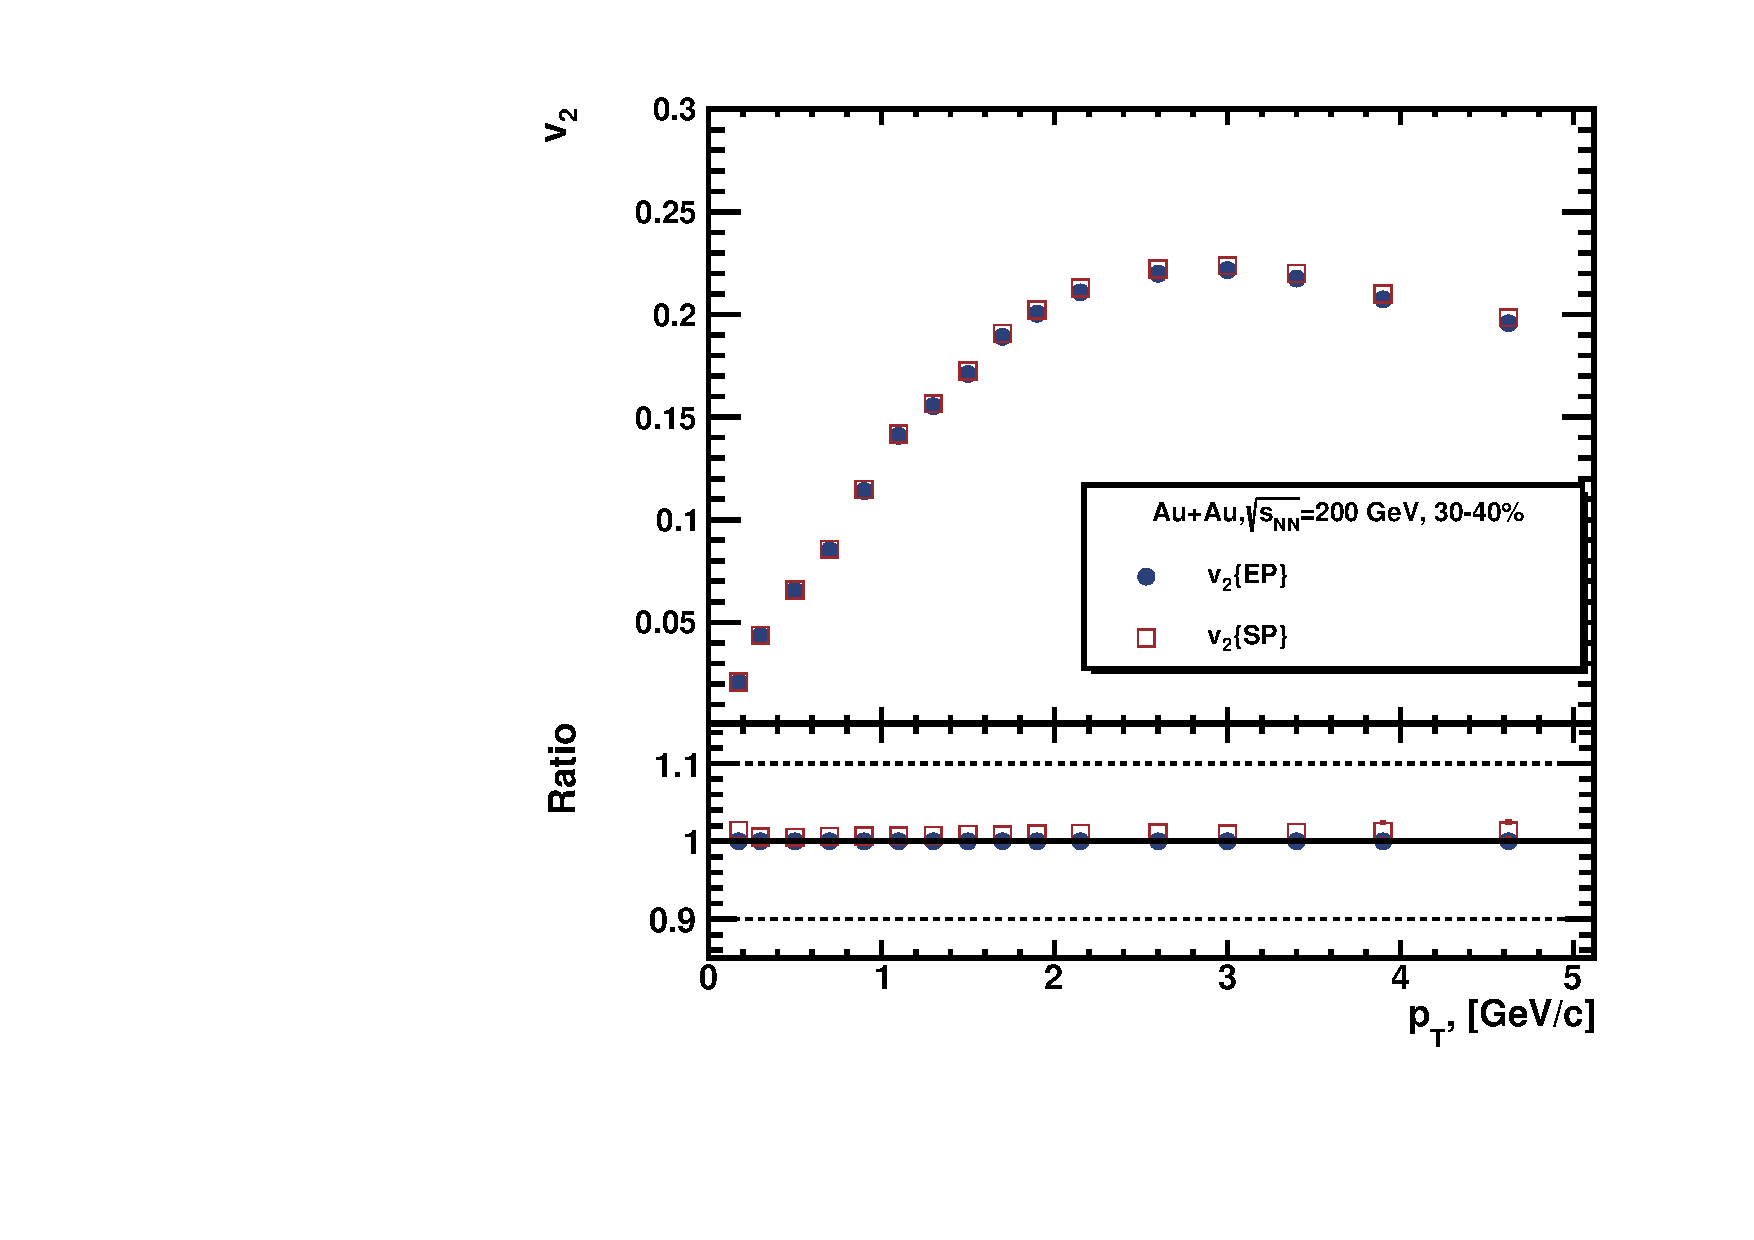
\includegraphics[width=1.\linewidth]{Figures/v2_CH_SP_pt_cent4.pdf}
        %\caption{b}
    \end{subfigure}
    \label{fig:v2_SP_CH}
    \caption{Charged hadron $v_2(p_T)$ for 5-10\% (upper left), 10-20\% (upper right), 20-30\% (bottom left) and 30-40 \% (bottom right) centrality classes in \AuAu\ collisions at \sNN\ = 200 GeV. Results gained with scalar product method were compared with the event-plane ones.}
\end{figure}

\FloatBarrier
\subsubsection{\BBC\ event-plane}

\begin{figure}[ht]
    \begin{subfigure}{.49\textwidth}
        \centering
        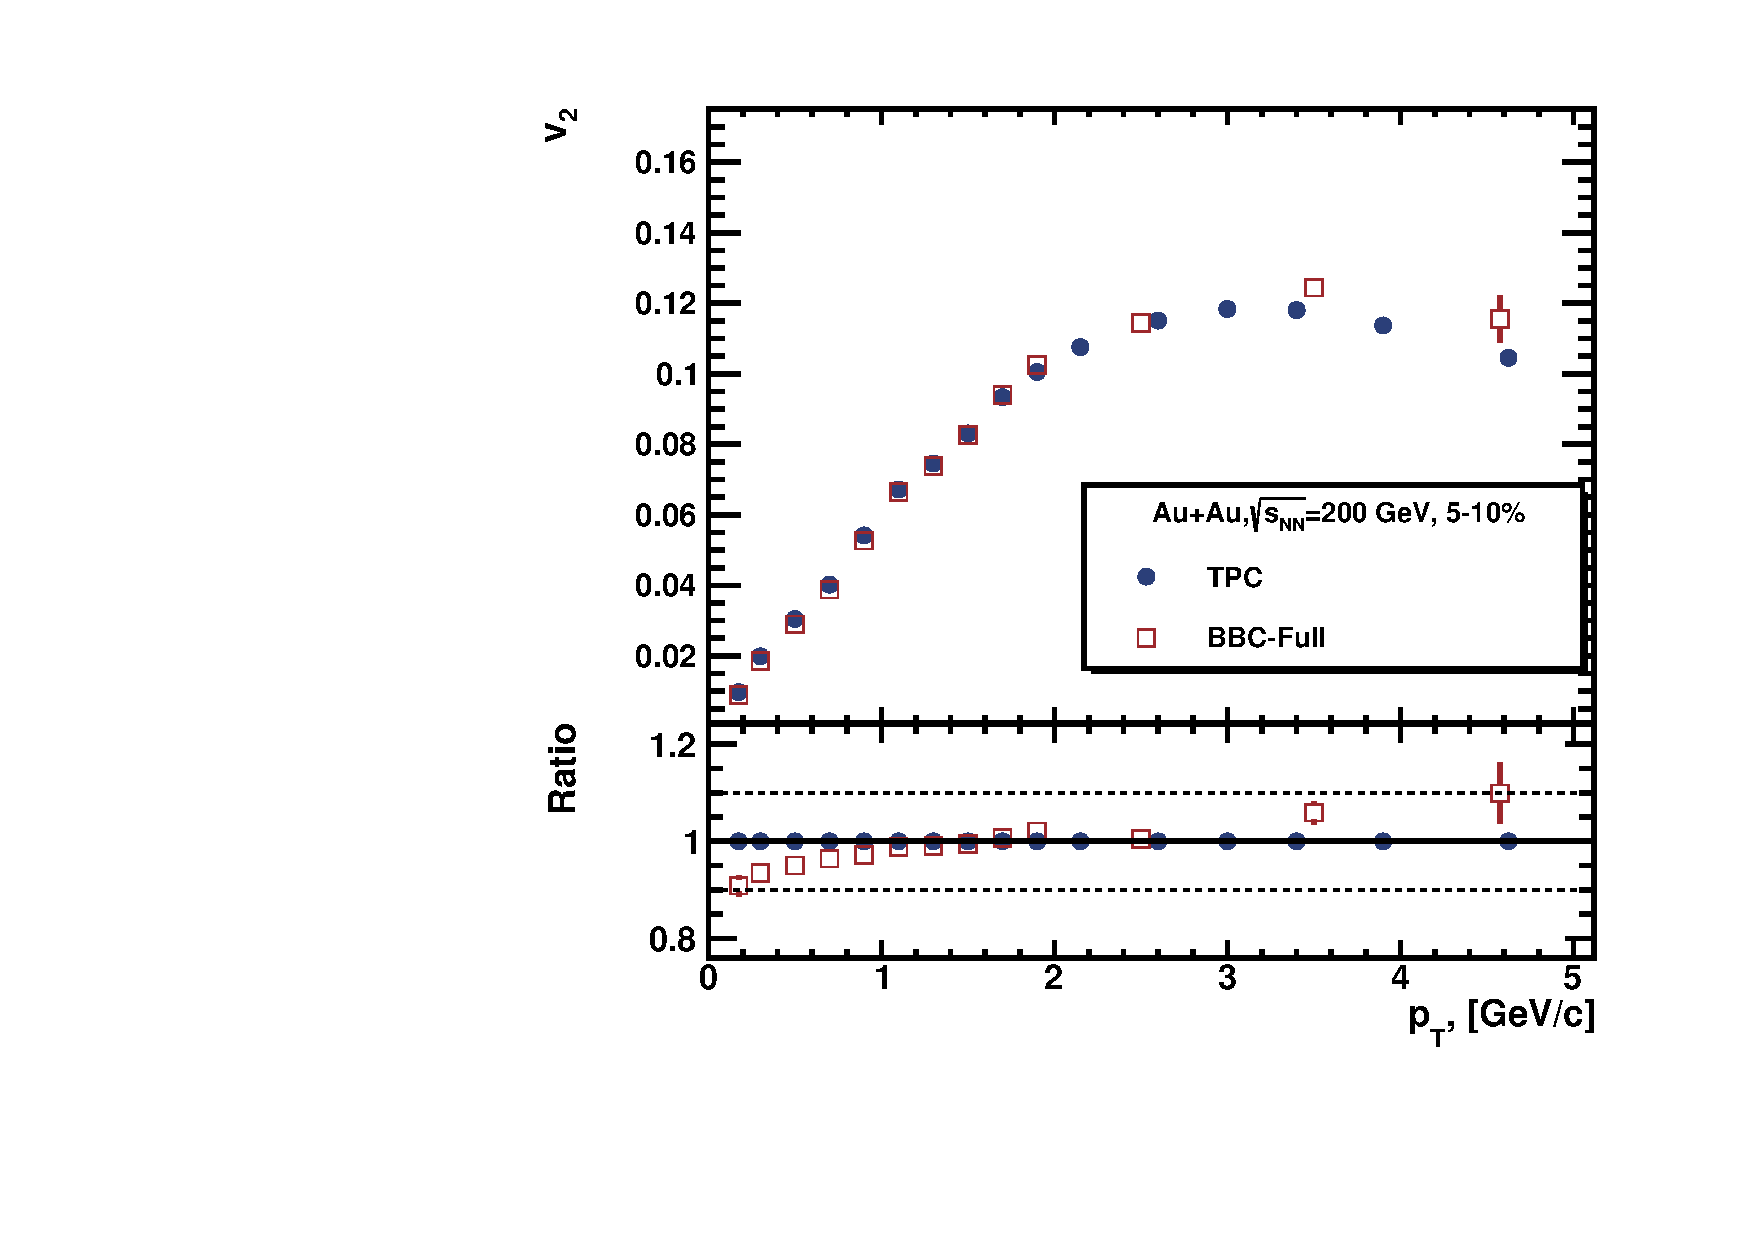
\includegraphics[width=1.\linewidth]{Figures/v2_CH_BBC_pt_cent1.pdf}
        %\caption{a}
    \end{subfigure}
    \begin{subfigure}{.49\textwidth}
        \centering
        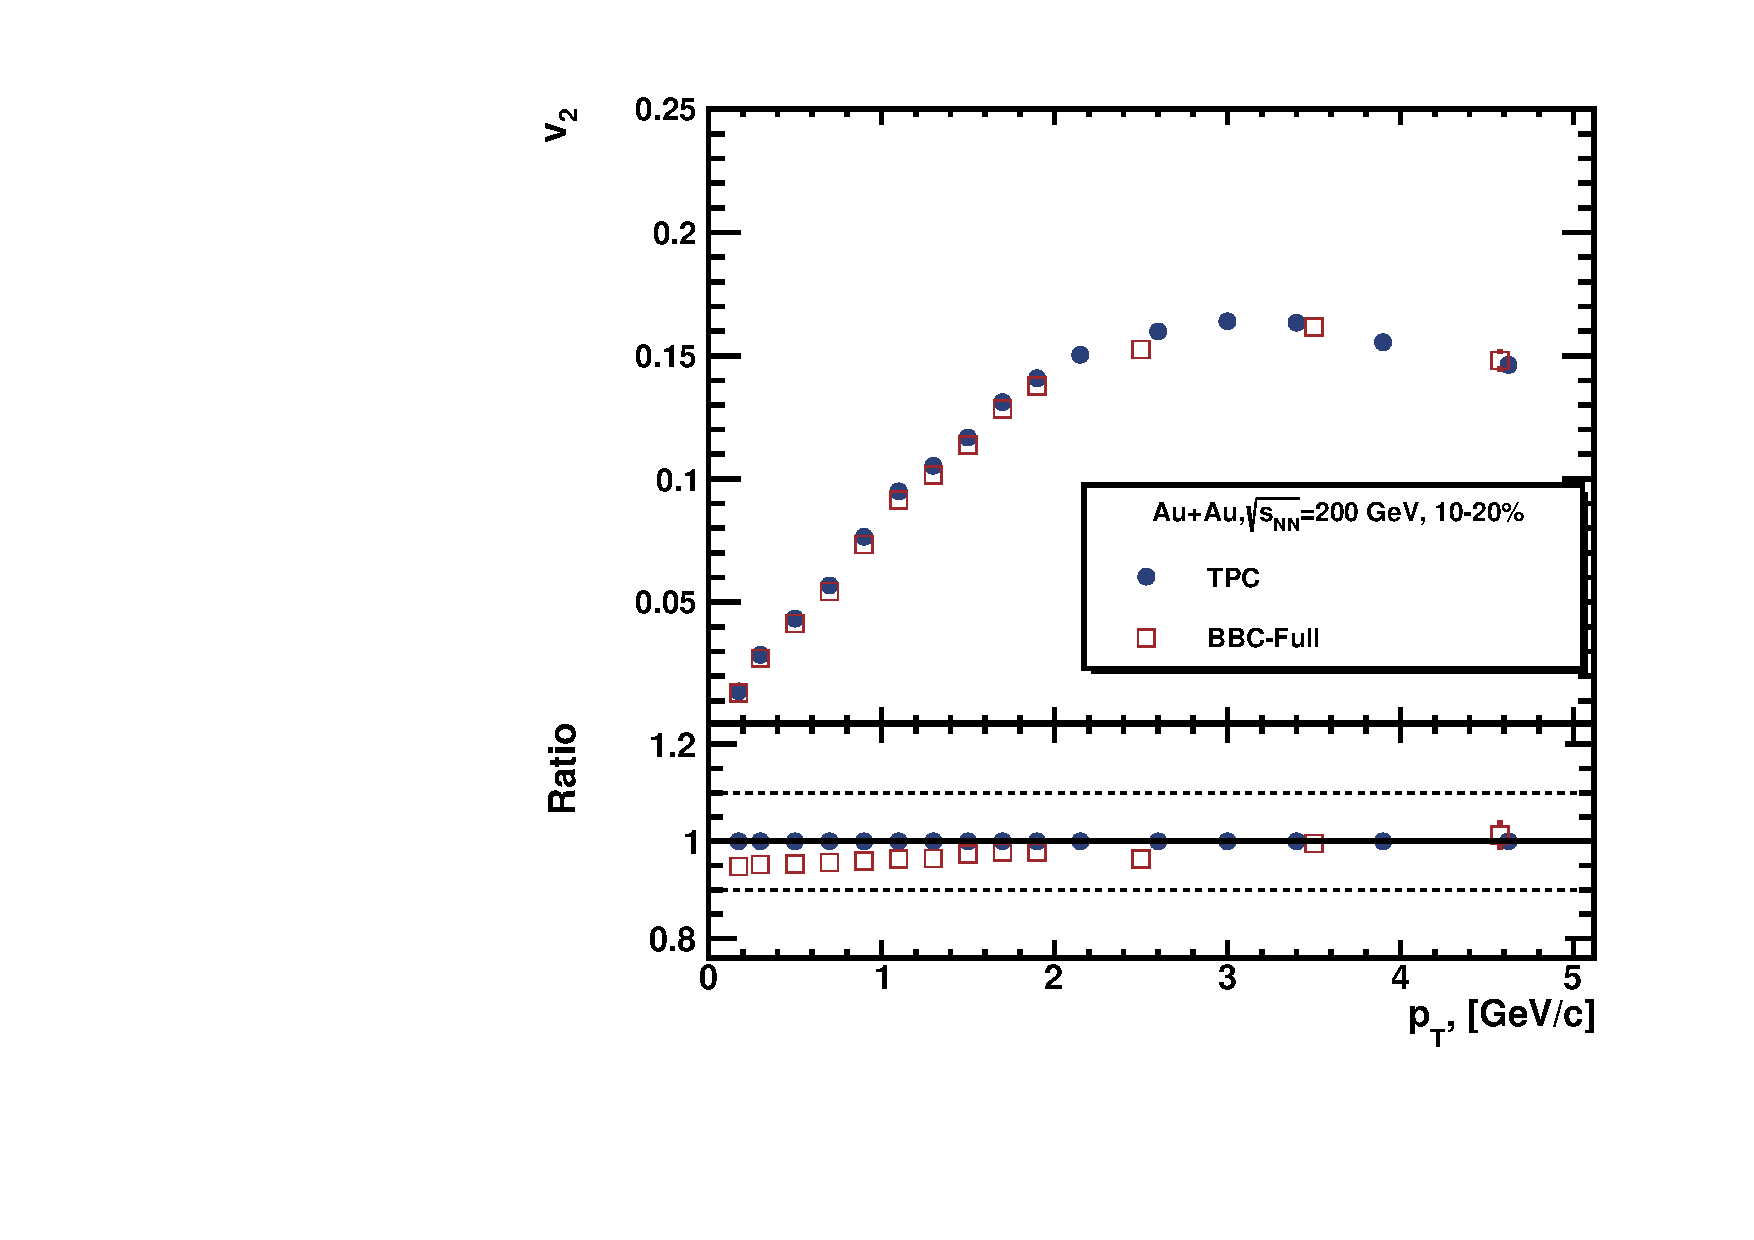
\includegraphics[width=1.\linewidth]{Figures/v2_CH_BBC_pt_cent2.pdf}
        %\caption{b}
    \end{subfigure}
    \\
    \begin{subfigure}{.49\textwidth}
        \centering
        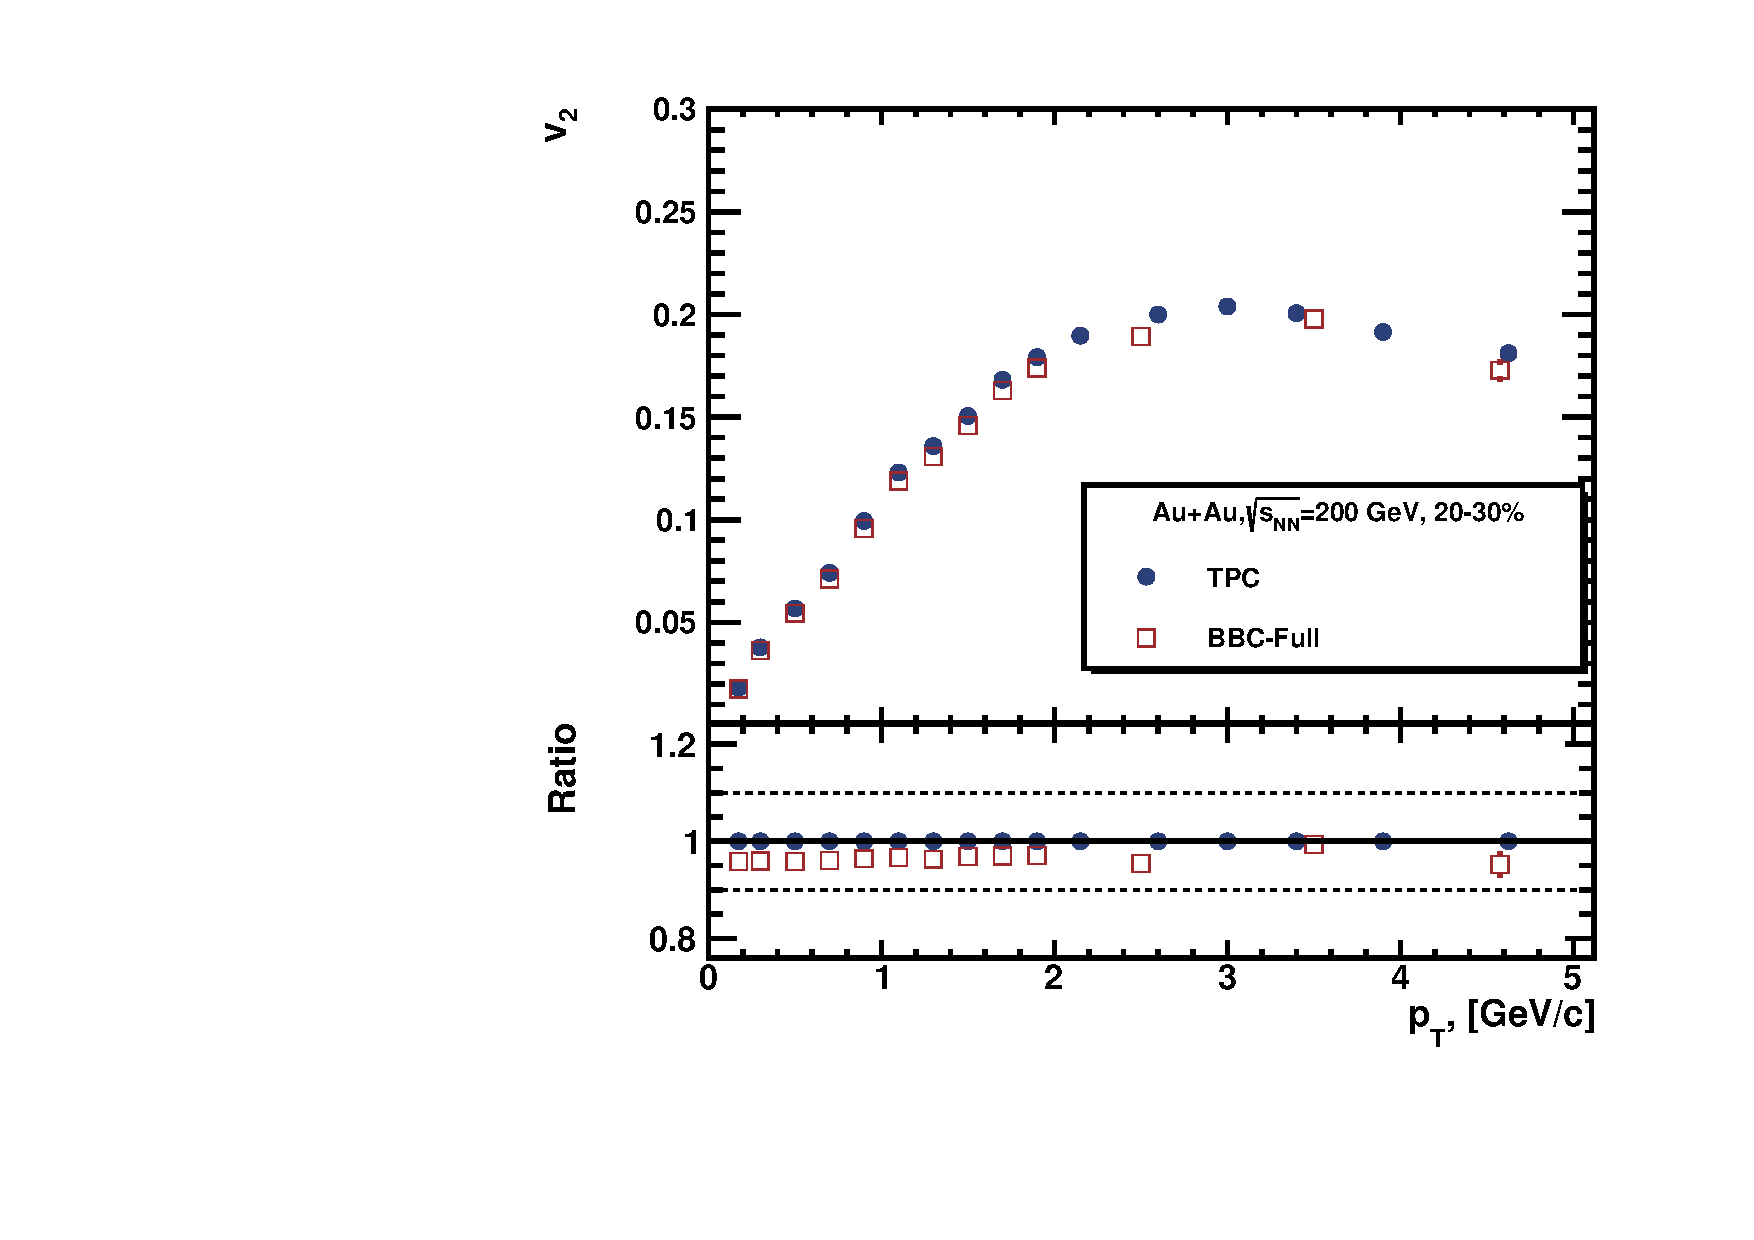
\includegraphics[width=1.\linewidth]{Figures/v2_CH_BBC_pt_cent3.pdf}
        %\caption{a}
    \end{subfigure}
    \begin{subfigure}{.49\textwidth}
        \centering
        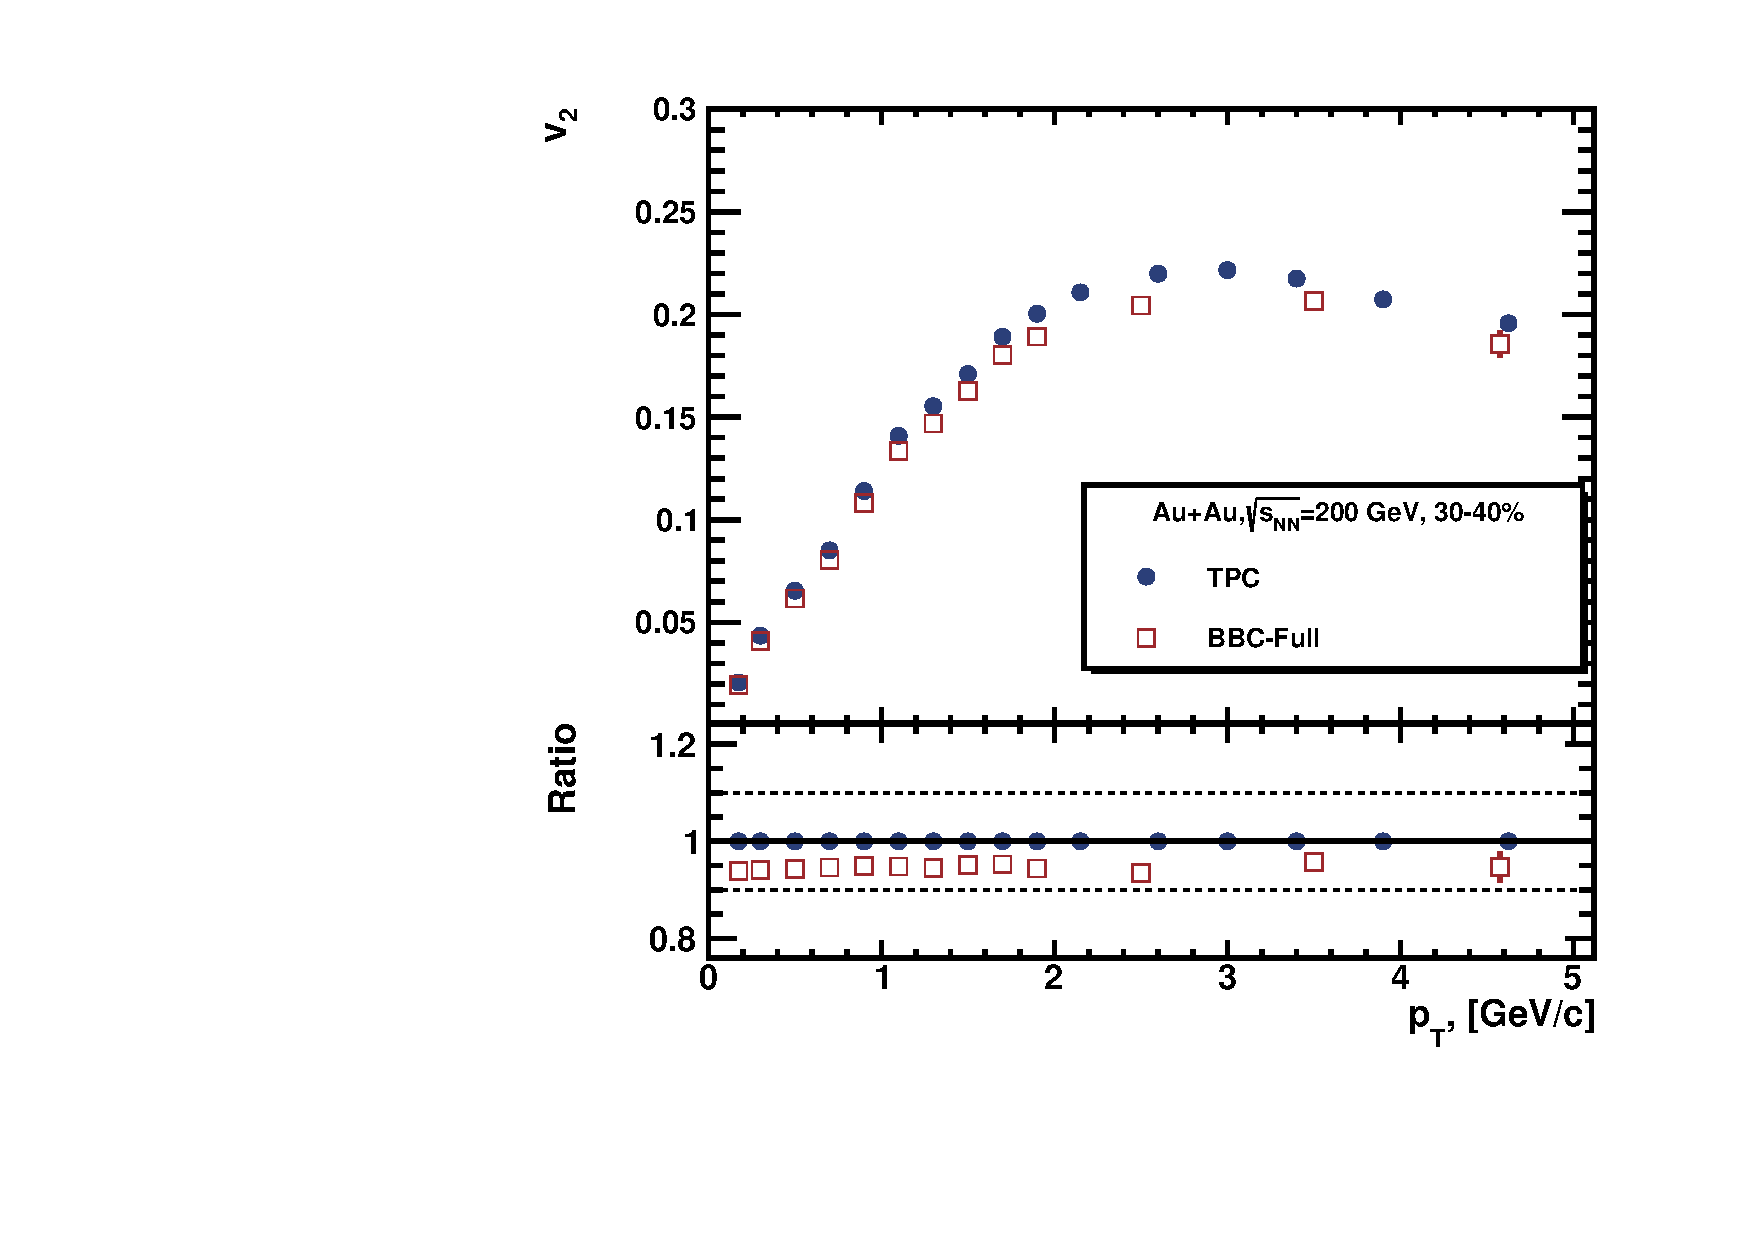
\includegraphics[width=1.\linewidth]{Figures/v2_CH_BBC_pt_cent4.pdf}
        %\caption{b}
    \end{subfigure}
    \label{fig:v2_BBC_CH}
    \caption{Charged hadron $v_2(p_T)$ for 5-10\% (upper left), 10-20\% (upper right), 20-30\% (bottom left) and 30-40 \% (bottom right) centrality classes in \AuAu\ collisions at \sNN\ = 200 GeV. Results gained with \BBC\ event-plane were compared with the \TPC\ event-plane ones.}
\end{figure}

\FloatBarrier
\subsubsection{3 sub-event method}

\begin{figure}[ht]
    \begin{subfigure}{.49\textwidth}
        \centering
        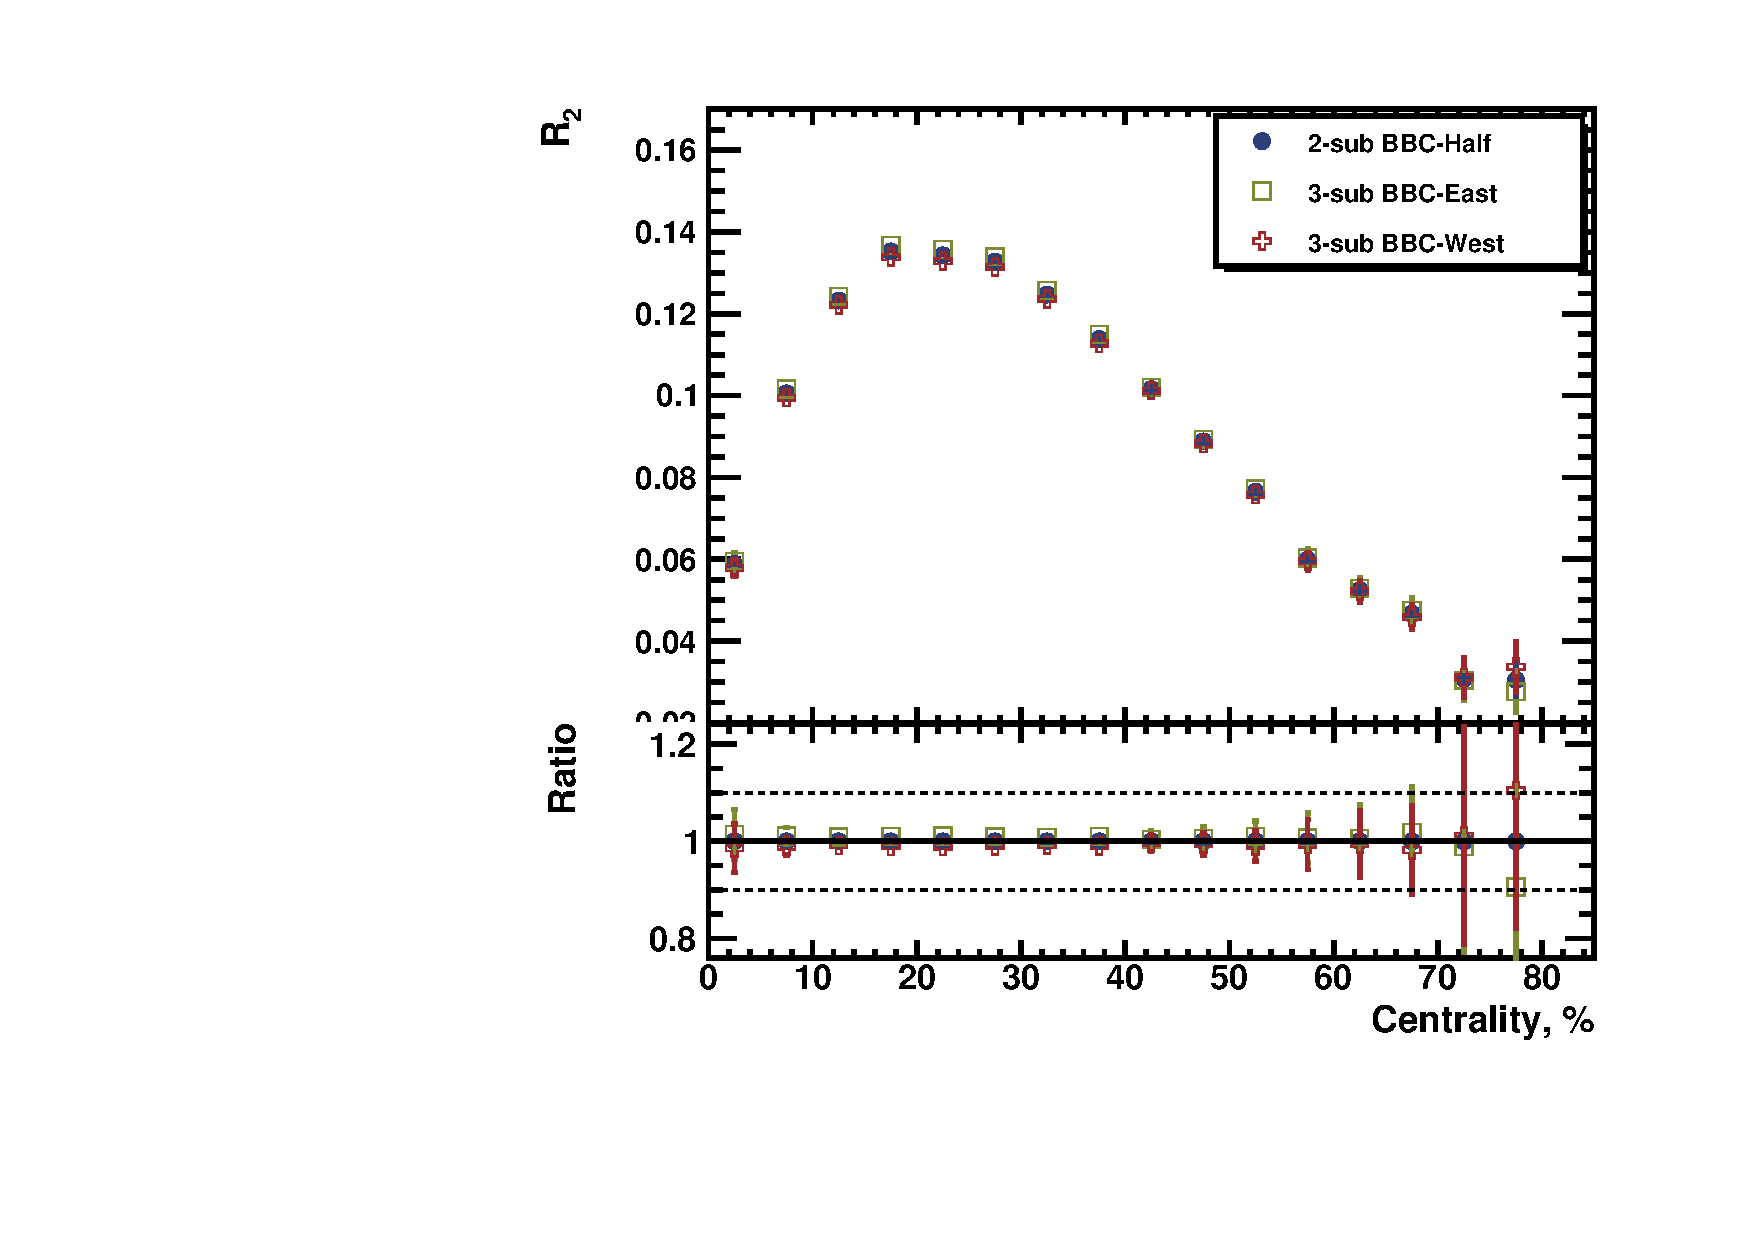
\includegraphics[width=1.\linewidth]{Figures/c_Res3sub2.pdf}
        %\caption{a}
    \end{subfigure}
    \begin{subfigure}{.49\textwidth}
        \centering
        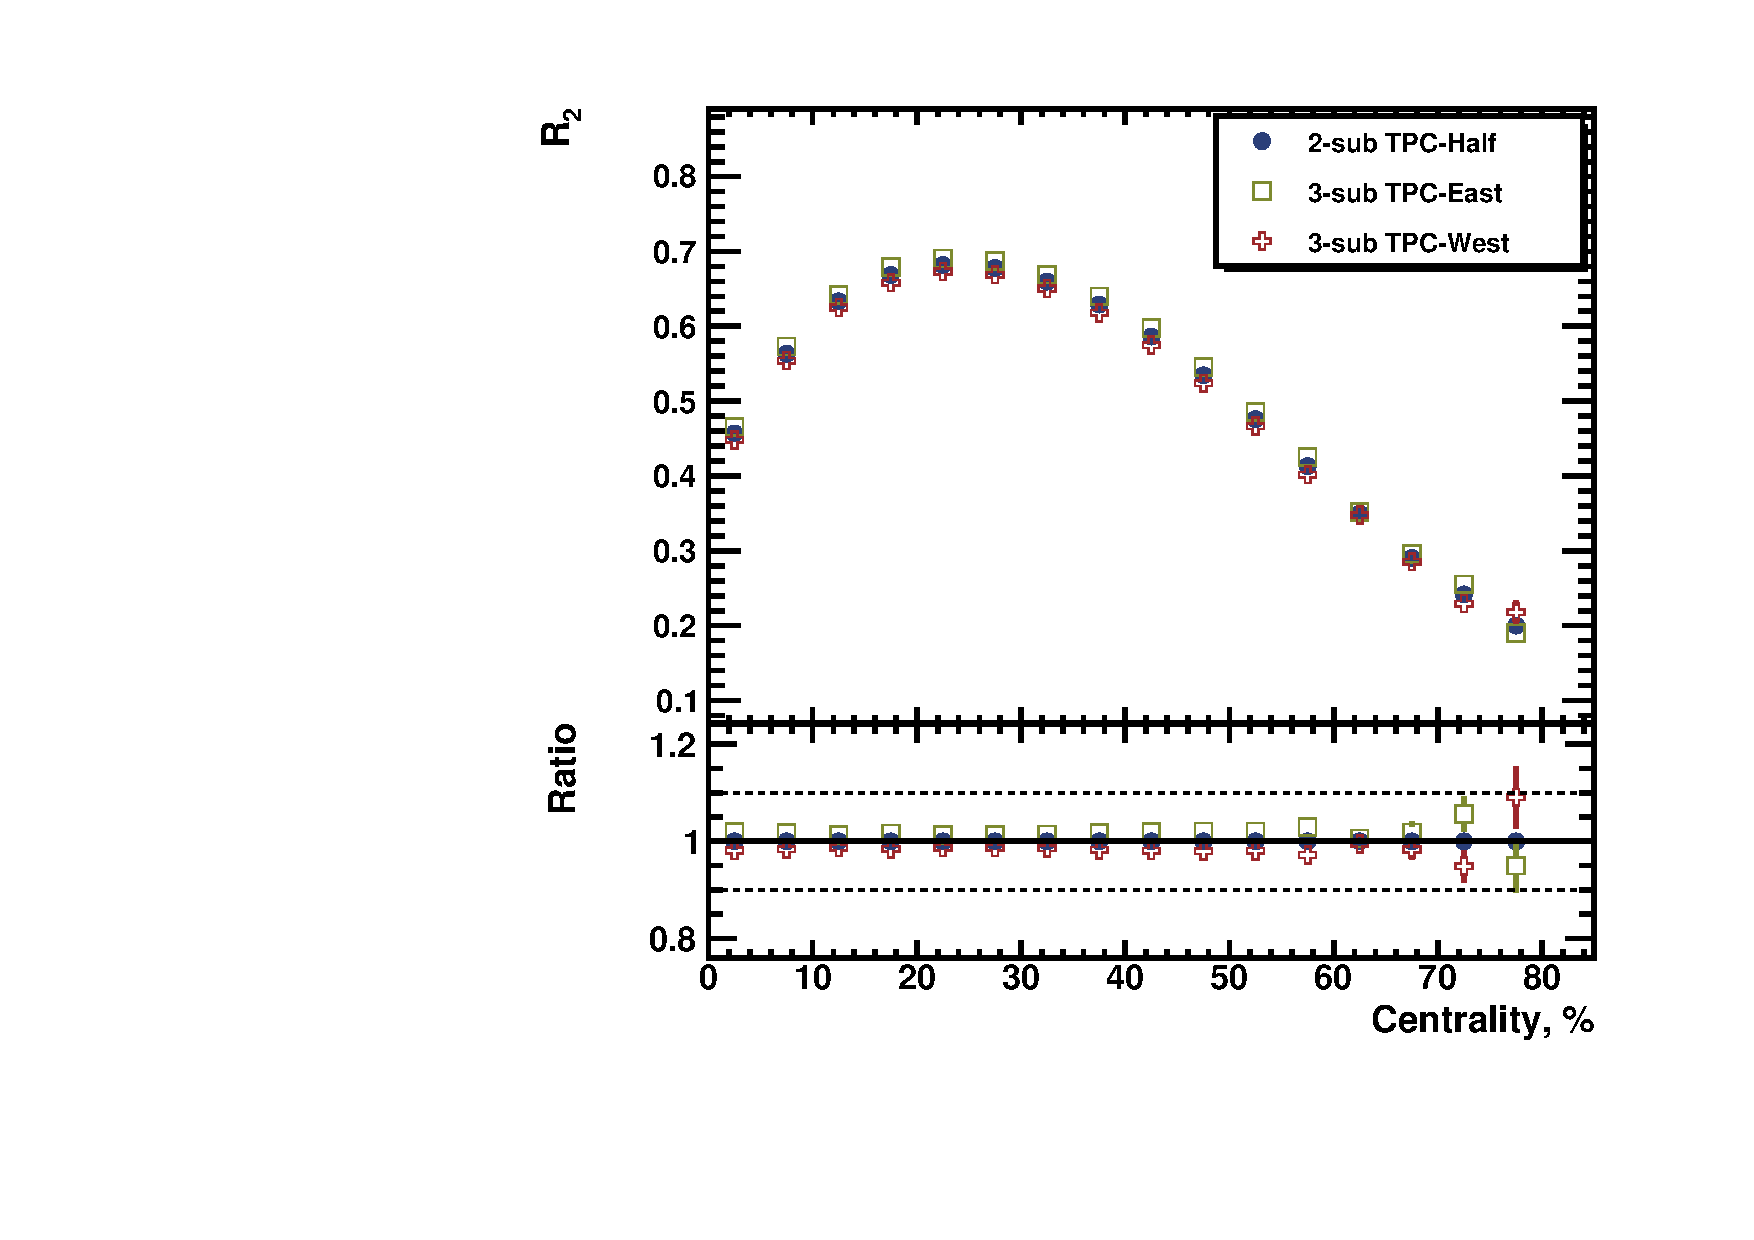
\includegraphics[width=1.\linewidth]{Figures/c_Res3sub3.pdf}
        %\caption{b}
    \end{subfigure}
    \label{fig:Res_3sub}
    \caption{The event-plane resolution correction factor calculated for \AuAu\ collisions at \sNN\ = 200 GeV using 3 and 2 sub-events as a function of centrality.}
\end{figure}